\documentclass{utm_report}

\addbibresource{references.bib}

% Table packages for comparative analysis tables
\usepackage{tabularx}
\usepackage{array}
\usepackage{longtable}
\usepackage{booktabs}
\usepackage{colortbl}
\usepackage[table]{xcolor}
\usepackage{makecell}
\usepackage{tikz}
\usepackage{pgfplots}
\usepackage{pgf-pie}
\usepackage{caption}

\captionsetup[figure]{labelsep=space}
\captionsetup[table]{labelsep=space}
\pgfplotsset{compat=1.18}

% Define Y only if not already provided by the class
\makeatletter
\@ifundefined{NC@find@Y}{\newcolumntype{Y}{>{\raggedright\arraybackslash}X}}{}
\makeatother

% \usepackage{showframe}    % DEBUG: Show margins & frames


\begin{document}

\hypersetup{pageanchor=false}

\newcommand{\ministryname}{MINISTRY OF EDUCATION AND RESEARCH OF THE REPUBLIC OF MOLDOVA}
\newcommand{\universityname}{Technical University of Moldova}
\newcommand{\facultyname}{Faculty of Computers, Informatics, and Microelectronics}
\newcommand{\departmentname}{Department of Software Engineering}
\newcommand{\reporttitle}{Internet of Things}
\newcommand{\reportsubtitle}{Wearable Inertial Gesture Interface for Surface-Independent Computer Control}
\newcommand{\reportyear}{2026}

\begin{titlepage}
    \centering

    % Ministry: bold, 12pt, tight line spacing (spacing -1 = single)
    {\fontsize{12pt}{12pt}\selectfont\bfseries \ministryname \\[4pt]}

    % University / Faculty / Department: bold, 14pt, tight line spacing
    {\fontsize{14pt}{14pt}\selectfont\bfseries
        \universityname \\[2pt]
        \facultyname \\[2pt]
        \departmentname \\
    }

    \vfill

    % Report title: bold, 20pt, centered
    {\fontsize{20pt}{22pt}\selectfont\bfseries \reporttitle \par}

    \vspace{10pt}

    % Report subtitle: bold, 16pt, centered
    {\fontsize{16pt}{18pt}\selectfont\bfseries \reportsubtitle \par}

    \vfill

    % Students / Coordinator block: bold, 12pt, right-aligned
    \hfill
    \begin{tabular}{ll}
        \textbf{Students:}    & \textbf{Chicu Andrei, FAF-233} \\
                              & \textbf{Cobzari Ion, FAF-233} \\
                              & \textbf{Crudu Alexandra, FAF-233} \\
                              & \textbf{Gurduza Mihai, FAF-233} \\
                              & \textbf{Moraru Patricia, FAF-233} \\[12pt]
        \textbf{Coordinator:} & \textbf{Malîi Antonela, university assistant} \\
    \end{tabular}

    \vfill

    % City and year: bold, 12pt, centered
    {\fontsize{12pt}{14pt}\selectfont\bfseries Chișinău, \reportyear \par}

\end{titlepage}
\chapter*{ABSTRACT}
\thispagestyle{empty}

The project report titled "AirGlove" was developed by students Chicu Andrei, Cobzari Ion, Crudu Alexandra, Gurduza Mihai, and Moraru Patricia at the Technical University of Moldova. It is written in English and contains an introduction, 5 chapters (Problem Definition \& Analysis, Domain Analysis, Proposed Solution, Comparative Analysis, Target Audience \& Stakeholders), a list of figures, a list of tables, bibliography, and appendices.

This report examines the limitations of conventional mouse and touchpad interaction in scenarios where a stable surface is unavailable, uncomfortable, or impractical, and frames the core problem, goals, and constraints for a surface-independent pointing solution. Building on this, the domain analysis reviews inertial pointing and wearable interaction approaches from both research and industry, highlighting recurring issues such as drift, user-to-user variability, and the need for robust mapping strategies. The proposed solution then introduces the AirGlove prototype, which combines an ESP32 microcontroller with an MPU6050/MPU6500 IMU and functions as a Bluetooth HID device to improve portability and reduce reliance on USB dongles commonly used by commercial air mice. Implementation choices are motivated by the full mid-air control pipeline: sensor fusion, smoothing and filtering, dead zones, gain shaping, and clutching; emphasizing that stability and usability depend on end-to-end processing rather than raw orientation estimation alone. A comparative analysis (SWOT and structured comparison table) positions the prototype against commercial products and research prototypes, clarifying where it performs well (openness, customizability, wearable form factor) and where trade-offs remain, including calibration effort, precision expectations, power consumption, and drift. Finally, the target audience and stakeholders section connects these technical decisions to realistic usage contexts, especially presentation control and accessibility-oriented interaction, and outlines improvement directions aimed at increasing reliability, comfort, and robustness across different users and environments.

\textbf{Keywords: } wearable input device, air mouse, IMU, ESP32, Bluetooth HID, sensor fusion, accessibility, ergonomics

\tableofcontents

\clearpage

% List of figures
\addcontentsline{toc}{chapter}{\listfigurename}
\listoffigures 

% You can decide whether to put the LOF and LOT 
% on the same page or on different pages.
% If on the same page, use some spacing:
\vspace{1\baselineskip}

% List of tables
\addcontentsline{toc}{chapter}{\listtablename}
\listoftables 

\hypersetup{pageanchor=true}

\addcontentsline{toc}{chapter}{INTRODUCTION}
\chapter*{INTRODUCTION}

Most computer interaction assumes a stable desk and a surface-based pointing device. In many real situations like presentations, classrooms, mobile work, or standing use, a mouse or touchpad is inconvenient or uncomfortable, and long sessions can also cause fatigue. These limitations motivate surface-independent pointing, where cursor control is achieved through mid-air motion rather than contact with a desk.

AirGlove is a wearable air-mouse prototype that explores this approach using accessible, low-cost components. Hand motion is captured by an inertial measurement unit (IMU) and translated into cursor movement and click actions, enabling basic computer control without a flat surface. The prototype uses an ESP32 microcontroller paired with an MPU6050/MPU6500 IMU and communicates with a host device as a Bluetooth Human Interface Device (HID). Beyond the hardware, the main challenge is achieving stable and usable cursor control despite noise, drift, and user variability, which requires an end-to-end processing pipeline (sensor fusion, smoothing and filtering, dead zones, gain shaping, and clutching).

This report defines the problem and constraints of mid-air pointing, motivates the selected design, and documents the current prototype. Chapter~1 (Problem Definition \& Analysis) outlines objectives and limitations. Chapter~2 (Domain Analysis) reviews research and commercial solutions to extract practical design lessons. Chapter~3 (Proposed Solution) describes the system architecture and interaction pipeline. Chapter~4 (Comparative Analysis) positions AirGlove using a SWOT analysis and structured comparison table. Chapter~5 (Target Audience \& Stakeholders) connects technical choices to realistic use cases and highlights future improvement directions. Appendices provide supporting material referenced throughout the report.
\chapter{DOMAIN ANALYSIS}

\section{Problem Definition \& Analysis}

This section establishes the problem addressed by the present work and analyses it across four complementary dimensions: epidemiological burden, biomechanical load, accessibility mismatch, and interaction-bandwidth constraint. Each dimension is examined with reference to peer-reviewed evidence, with the objective of demonstrating that classical computer input methods produce a measurable ergonomic and inclusion gap that justifies investigation of a wearable, movement-native alternative. The chapter concludes with a formal problem statement that synthesises the findings of the analysis.

\subsection{Problem Definition}

Classical computer input devices, particularly mice and trackpads, remain the dominant interaction mechanism in office, educational, and home-computing contexts. Their performance advantages for precision pointing are well established; however, they rely on prolonged static postures, repetitive micro-movements, and environmentally constrained fine-motor control. These properties increasingly conflict with contemporary computing patterns, where users interact for longer durations, in more diverse physical contexts, and with more heterogeneous physical abilities.

The long-horizon trajectory of this burden is summarised in Figure~\ref{fig:msd_global_trend}, which shows the growth in global prevalence estimates and projections.
\begin{figure}[ht!]
  \centering
  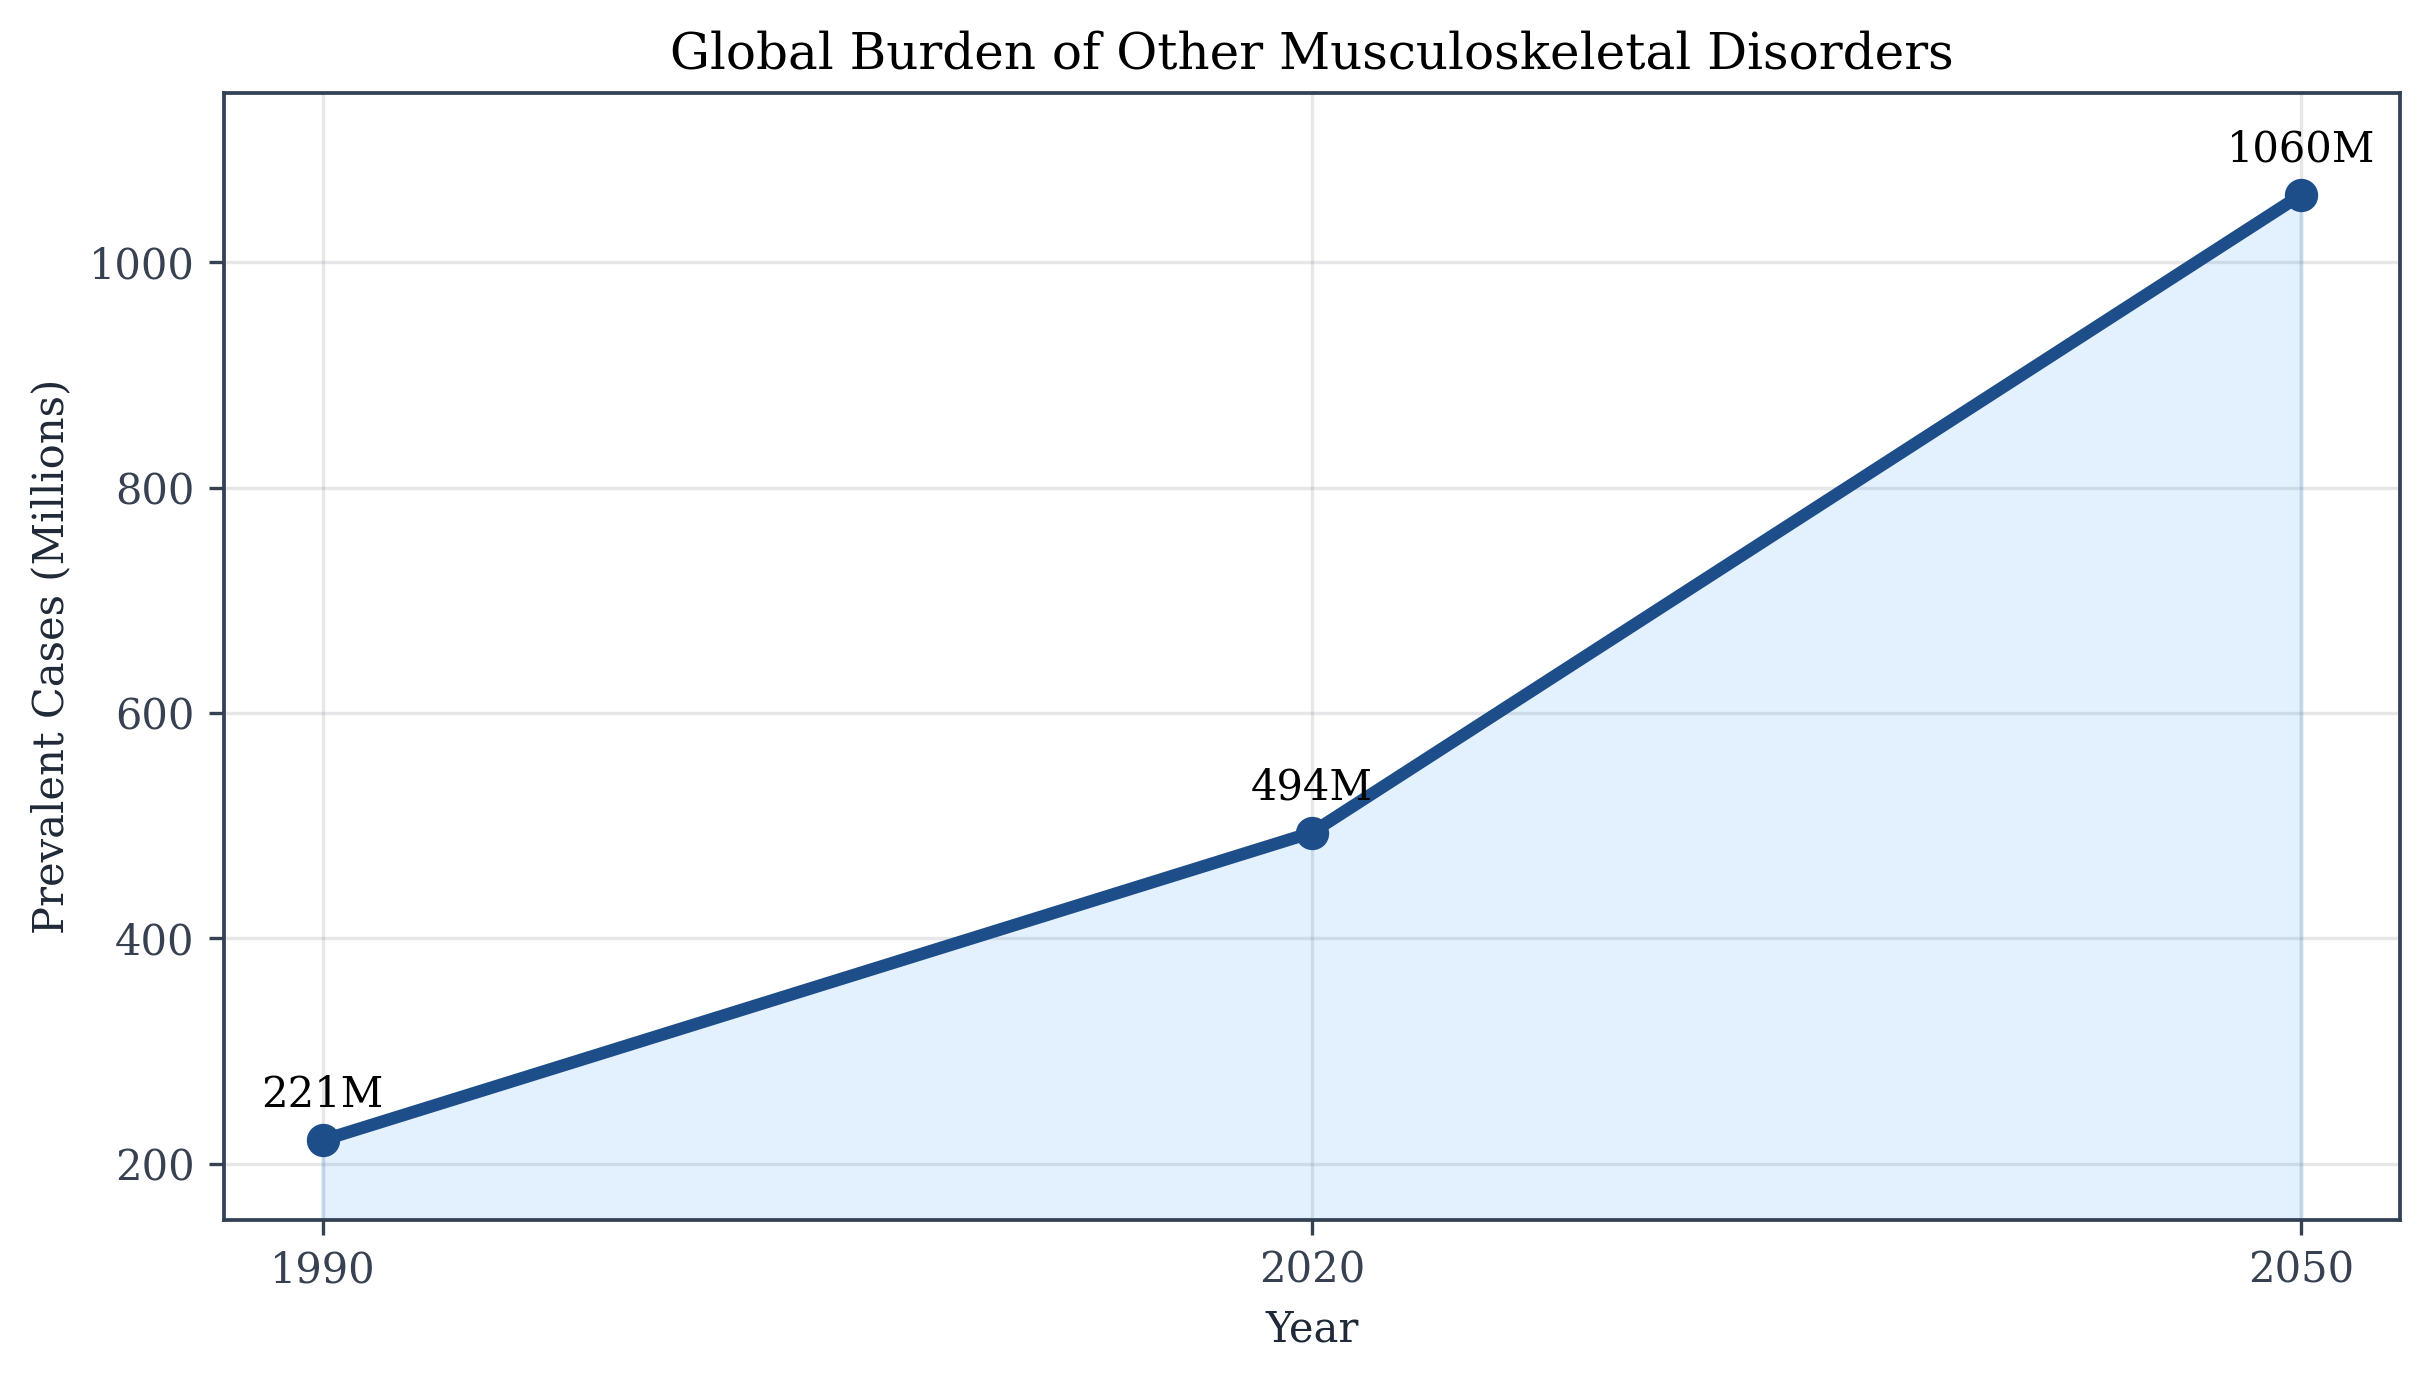
\includegraphics[width=0.7\linewidth]{img/ch1_msd_burden_trend.png}
  \caption{Global Growth in Other Musculoskeletal Disorder Cases (1990--2050 Projection)}
  \label{fig:msd_global_trend}
\end{figure}

Therefore, the core problem is not only discomfort at the individual level, but a systemic mismatch between the assumptions embedded in classical input devices and the current human, clinical, and contextual realities of computer use.

\newpage
The health burden associated with this interaction model is substantial. A systematic review found work-related musculoskeletal disorder (MSD) prevalence among computer users ranging from 33.8\% to 95.3\% depending on cohort and diagnostic approach~\cite{demissie2024wrmsd}. At population scale, the burden is amplified: musculoskeletal conditions affect approximately 1.71~billion people globally~\cite{who2022musculoskeletal}, and disability affects roughly 1.3~billion people~\cite{who2022disability}. Long-term trend data indicate that this is not a static issue; the Global Burden of Disease analysis reports a 123.4\% increase in MSD cases from 1990--2020, with projections continuing upward to 2050~\cite{gbd2023othermsd}.

\subsection{Problem Analysis}

The causes and impacts of the identified problem are multifactorial and can be analysed across four dimensions: biomechanical load, accessibility mismatch, environmental dependency, and interaction-bandwidth limitation.

\subsubsection{Biomechanical Load and Injury Risk}

Biomechanical studies identify several concurrent stressors during classical mouse use: forearm pronation, wrist extension, static muscular activation, and repetitive click-force execution. In controlled comparisons, classical mouse posture requires approximately 42$^\circ$ of forearm pronation, while alternative ergonomic configurations reduce this value and the associated extensor-muscle activation~\cite{quemelo2013vertical}. Wrist extension commonly exceeds 30$^\circ$ across multiple device designs~\cite{feathers2013alternative}, and carpal-tunnel pressure in symptomatic users has been measured at levels substantially above established neurophysiological risk thresholds during mousing tasks~\cite{schmid2015vertical}.
\begin{figure}[H]
  \centering
  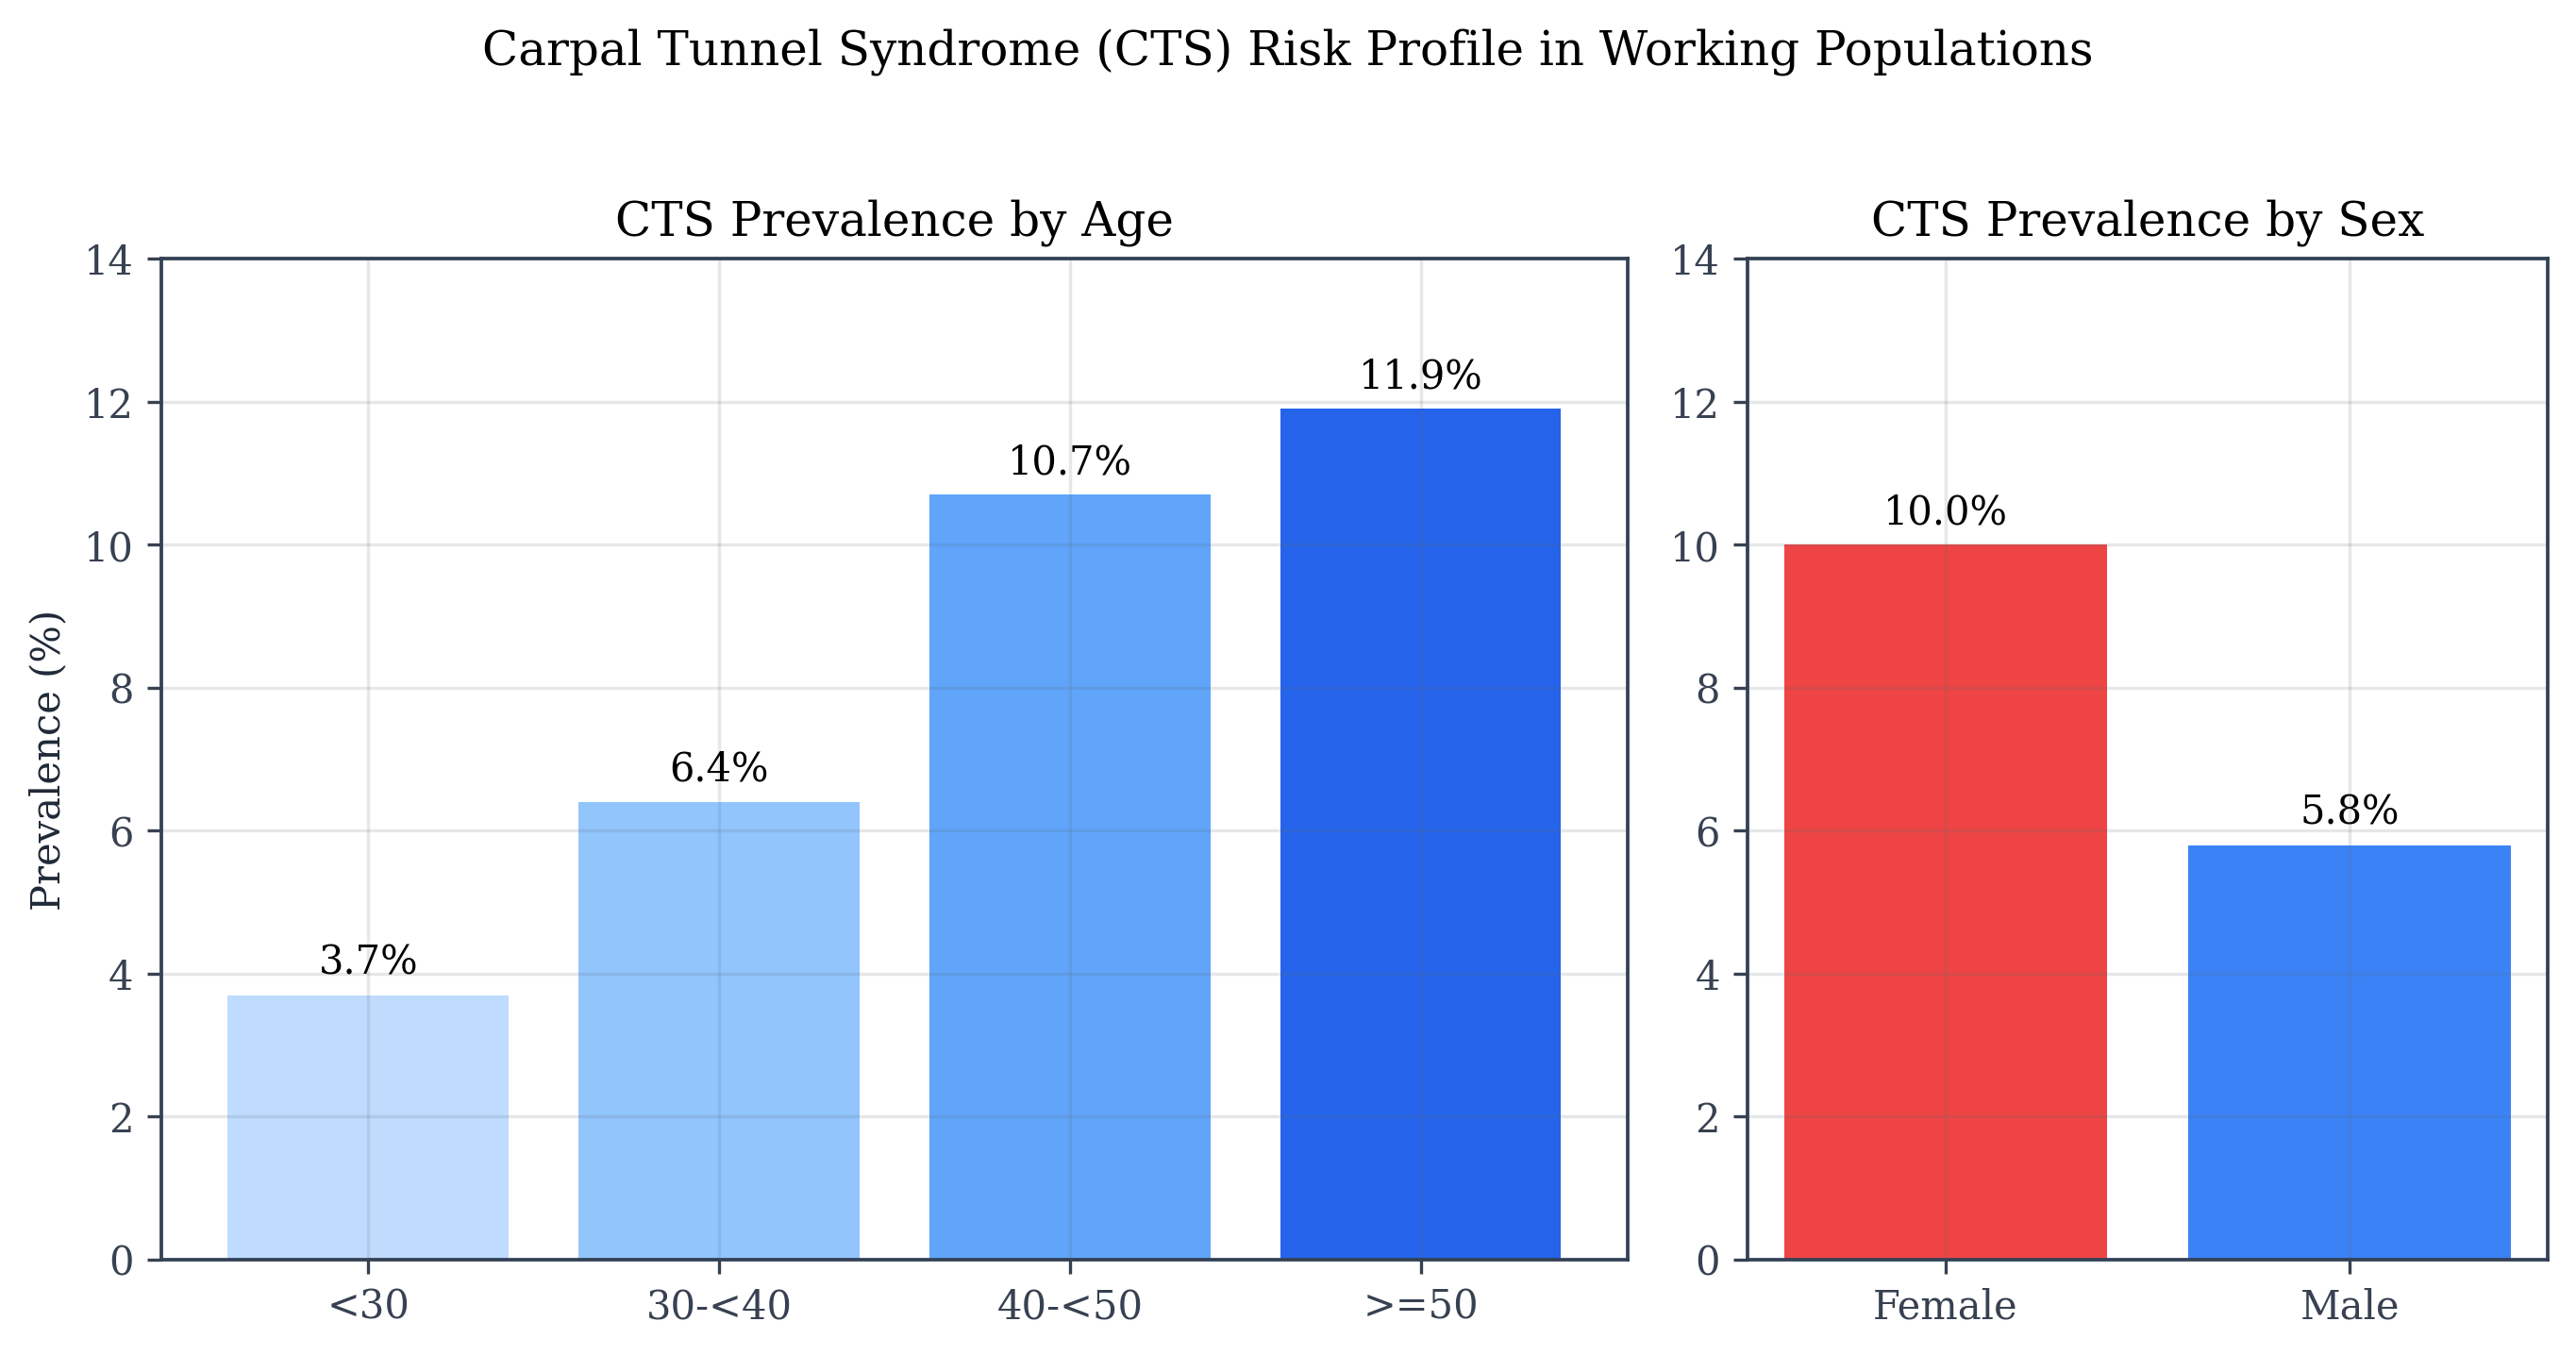
\includegraphics[width=0.7\linewidth]{img/ch1_cts_risk_profile.png}
  \caption{CTS Prevalence Profile by Age and Sex in Working Populations}
  \label{fig:cts_risk_profile}
\end{figure}

CTS burden is also patterned by demographic factors, with higher prevalence in older age groups and among female workers, as shown in Figure~\ref{fig:cts_risk_profile}. This distribution supports prioritising high-exposure and clinically vulnerable user segments in problem framing.

The profile indicates that occupational risk is not uniformly distributed and should be interpreted with exposure conditions, age structure, and workforce composition in mind. This supports prioritising high-intensity computer-use settings and user groups with elevated baseline vulnerability during requirements framing.

Exposure-time findings reinforce the clinical concern. Mouse use above 50\% of work time is associated with significantly higher odds of hand and wrist symptoms~\cite{andersen2003mouse}, and prolonged weekly exposure is linked to forearm pain risk~\cite{thomsen2008mouse}. For carpal tunnel syndrome (CTS), pooled occupational data report 7.8\% prevalence and an incidence rate of 2.3 cases per 100 person-years~\cite{dale2013cts}. Subclinical effects precede formal diagnosis: one study identified electrophysiological median-nerve entrapment in 34.8\% of asymptomatic long-term mouse users~\cite{ali2010median}.

\subsubsection{Accessibility Mismatch and Exclusion Risk}

The classical pointer-click paradigm presumes stable fine-motor control for both trajectory correction and click stabilisation. This assumption excludes many users with tremor, weakness, pain, or motor variability. The affected population is large: osteoarthritis alone affects approximately 595~million people globally~\cite{gbd2023oa}, and significant prevalence is documented across essential tremor~\cite{zheng2021essential}, cerebral palsy~\cite{mcintyre2022cp}, Parkinson's disease~\cite{maserejian2020parkinson}, and multiple sclerosis populations~\cite{lamers2016upperlimb}.

Empirical human-computer interaction (HCI) research identifies specific breakdown points in classical mouse interaction for motor-impaired users: precise target acquisition and click activation without cursor displacement~\cite{wobbrock2008goal}. In arthritis cohorts, 85\% of participants reported computer-use difficulties at considerable or very high levels~\cite{baker2009arthritis}. At societal level, these barriers align with observed digital-access disparities, including substantially lower device ownership rates among adults with disabilities~\cite{perrin2021disabilitytech}.

\subsubsection{Environmental Dependency and Contextual Inflexibility}

Classical mouse and trackpad systems are architecturally surface-dependent. Effective operation assumes access to a flat, stable workspace and a body posture compatible with sustained planar hand motion. This surface-availability assumption fails in many real-world use contexts, including standing presentations, bedside interaction, fieldwork, and ad hoc mobile workstations. The consequence is a contextual mismatch: computing is increasingly ubiquitous, yet primary input tools remain optimised for fixed-desk environments and cannot follow users into contexts where such environments are unavailable. This limitation is particularly relevant for the use cases that motivate the present work, where surface-independent, posture-flexible input is a core requirement.

\subsubsection{Interaction-Bandwidth Constraint}

Beyond health and accessibility, classical pointing interaction imposes a representational bottleneck by mapping rich hand-arm movement onto two-dimensional surface translation. Comparative pointing-performance studies have shown that gyroscopic spatial input currently trails mouse throughput, but remains functionally competitive and technically improvable~\cite{ramcharitar2017fitts}. This indicates that the problem is not an absence of alternatives, but the absence of an approach that jointly optimises ergonomics, accessibility, portability, and precision.

\begin{figure}[!hb]
  \centering
  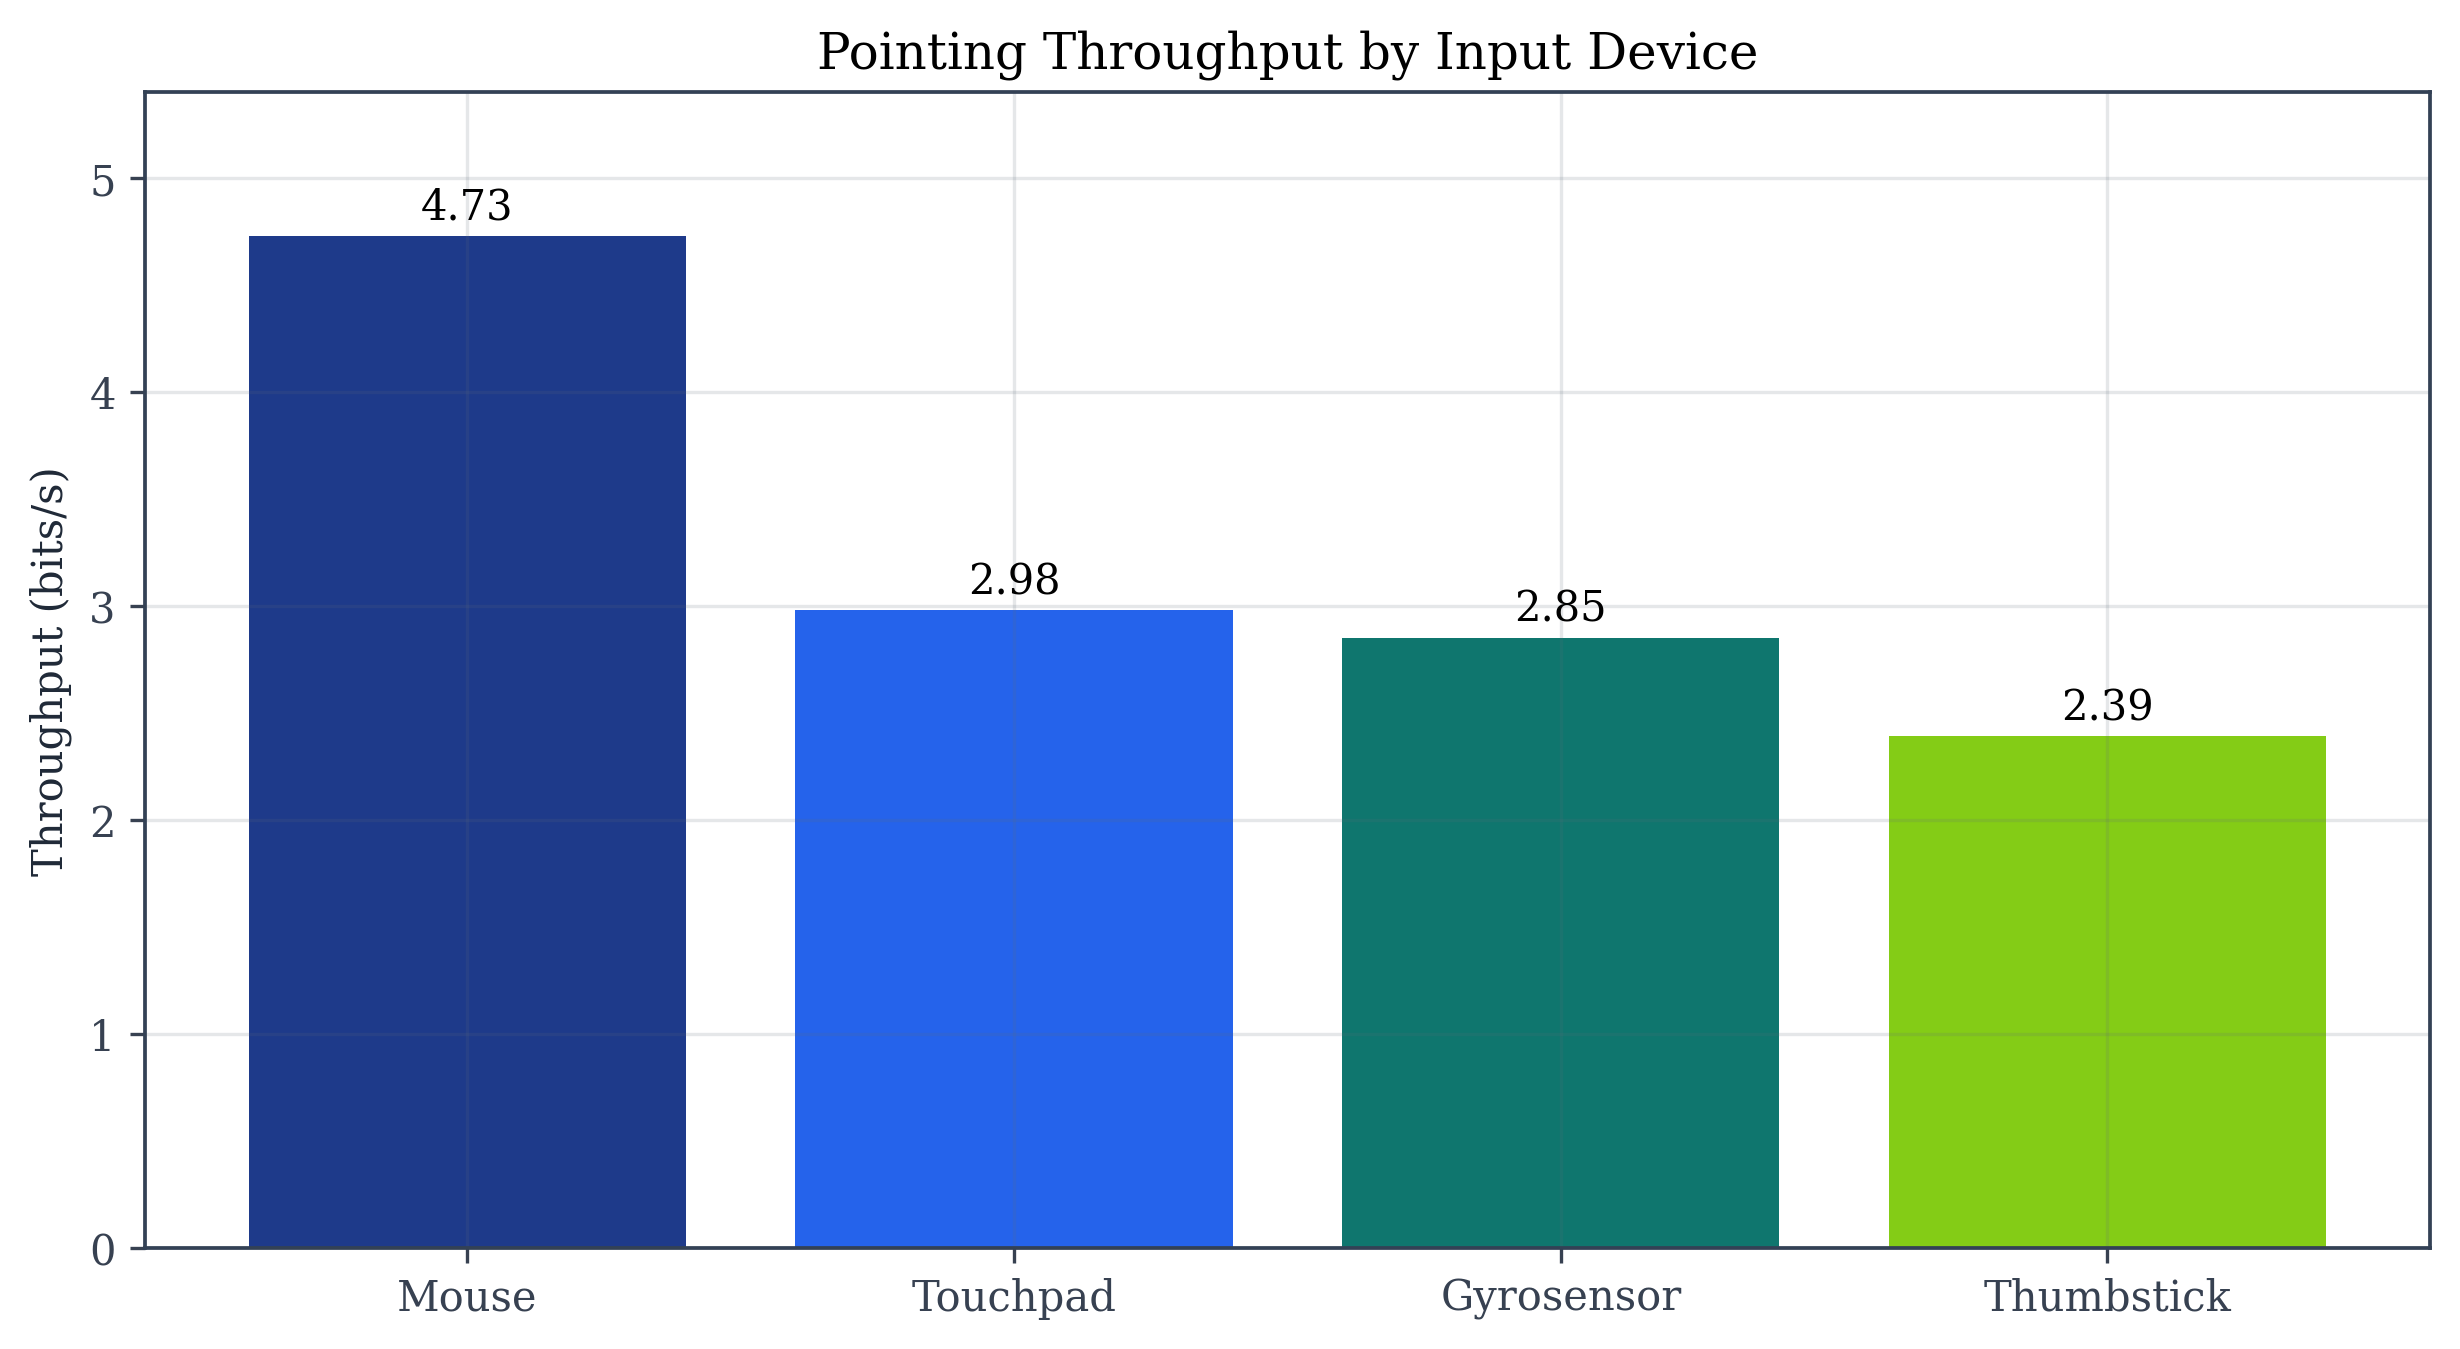
\includegraphics[width=0.7\linewidth]{img/ch1_input_throughput_comparison.png}
  \caption{Pointing Throughput Comparison Across Input Devices}
  \label{fig:throughput_comparison}
\end{figure}

Figure~\ref{fig:throughput_comparison} presents the reference throughput comparison used in this chapter and clarifies the current performance gap that motivates algorithmic and interaction-design refinement. Although the throughput gap remains meaningful, the comparison still positions gyroscopic interaction above some conventional controller modalities. This supports treating performance as an optimisation target rather than a hard feasibility barrier.

Appendix Table~\ref{tbl:problem_indicators} presents key quantitative indicators used to delineate the problem space and justify investigation of alternative input approaches. Taken together, these indicators justify the present work as a problem-driven intervention rather than a novelty-driven interface variant.

Following the above analysis, the following problem statement has been derived: Classical mouse- and trackpad-based interaction imposes cumulative biomechanical strain, depends on fixed planar workspaces, and inadequately accommodates motor variability across the user population, creating a demonstrable need for a wearable, movement-native input approach that improves ergonomic sustainability and accessibility while preserving functional pointing performance.

\section{Domain Analysis}

Pointing is a fundamental interaction primitive in graphical user interfaces, and even small efficiency gains can have a large cumulative usability impact because the action is repeated continuously in everyday computing. Traditional surface-based mice convert planar hand translation into stable cursor displacement with minimal drift, while touchpads and trackballs trade precision for compactness or portability. Air mice relocate pointing into free space: users rotate or move a handheld device and software maps that motion to cursor control. This shift changes both engineering constraints and human factors. Without a mechanical surface, orientation and motion must be inferred from noisy embedded sensors, and the user must sustain a mid-air posture that can become fatiguing over longer sessions.

 

\subsection{Domain Scope, Positioning, and Modality Trade-offs}

Air-mouse systems lie at the intersection of embedded sensing, control filtering, interaction design, and ergonomic evaluation. Any analysis in this domain must begin by acknowledging that the performance target is still set by conventional desktop pointing devices. Foundational comparative studies established the superior accuracy-speed balance of the mouse relative to rate-controlled alternatives~\cite{card1978evaluation}. Later methodological work in HCI and ergonomics provided standardized ways to evaluate non-keyboard devices through movement-time/error trade-offs and throughput-driven interpretation aligned with ISO-style test paradigms~\cite{iso9241_9_2000}. Therefore, the question is not whether air pointing can function technically; it is whether it can deliver stable, predictable, low-effort control under realistic constraints.

From a systems perspective, contemporary air-pointing technologies are commonly grouped into three modality families. The first is inertial tracking, where an embedded IMU provides angular-rate and acceleration data used for estimating orientation and generating cursor commands. The second is vision-based tracking, where cameras infer hand pose or device pose from image features. The third is infrastructure-assisted tracking, where external hardware such as optical markers, base stations, or dedicated emitters provides absolute spatial references. Each family solves a different subset of problems while introducing its own constraints.

Inertial tracking is the most suitable choice for low-cost Arduino-class projects because it is self-contained and does not require environmental setup. It supports mobile operation and rapid prototyping with affordable hardware. Its core challenge is drift and zero-state instability, especially over longer sessions. Vision-based tracking can provide strong absolute information in controlled settings, but performance is sensitive to lighting, occlusion, background complexity, camera placement, and host compute. Infrastructure-assisted systems can be highly accurate and drift-resistant, but they are less appropriate for compact educational or consumer prototypes due to setup complexity and cost.

For this project context, inertial sensing best matches the design objective: a self-contained, low-cost, embedded artifact that can emulate a standard pointing device. The Arduino ecosystem directly supports HID mouse behavior on compatible boards through the Mouse API~\cite{arduino_mouse_reference}, while BLE-HID implementation patterns for wireless scenarios are documented in embedded vendor ecosystems~\cite{nordic_hids_mouse_sample}. This availability allows the project to focus on meaningful domain problems (fusion quality, control mapping, and usability metrics) instead of spending disproportionate effort on external infrastructure.

A second positioning point concerns scientific defensibility. In educational prototypes, it is common to prioritize ``it works'' demonstrations, but that is insufficient for a rigorous domain chapter. A proper state-of-the-art analysis must connect technological feasibility to measurable user-level quality: stability at rest, correction latency, click reliability, and endurance under repeated use. This requirement motivates both the engineering decisions and the structure of the evaluation framework later in this chapter.

\subsection{Inertial Sensing, Sensor Fusion, and Robust Cursor Behavior}

An IMU does not directly provide orientation in a form suitable for cursor control. It provides raw measurements with different dynamics and error sources. The gyroscope provides angular velocity with high short-term responsiveness but accumulates integration error and bias over time. The accelerometer captures gravity and linear acceleration simultaneously, which makes tilt correction possible but only under assumptions about motion dynamics. If a magnetometer is available, yaw estimation can be constrained using Earth's magnetic field, but local magnetic disturbances, hard-iron/soft-iron effects, and imperfect calibration can degrade reliability.

These characteristics make sensor fusion mandatory rather than optional. Embedded implementations frequently use Madgwick- and Mahony-class methods because they offer a practical compromise between numerical stability and computational efficiency~\cite{madgwick2010efficient,mahony2008nonlinear}. In this domain, algorithm choice is not an abstract theoretical preference: it directly determines whether control feels stable enough for target acquisition and selection. On constrained boards, fusion also interacts with sampling-rate consistency, loop timing jitter, and available floating-point performance, which means implementation discipline is as important as formula selection.

A common misconception in early prototypes is that ``better absolute orientation'' automatically produces better pointing. In practice, user-perceived control quality depends on the full control chain: sampling, filtering, mapping, dead-zone logic, gain shaping, click handling, and clutching. Residual bias that seems numerically small can still produce visible cursor creep at rest. Likewise, aggressive smoothing that reduces jitter can introduce lag that harms corrective aiming. Therefore, the appropriate design objective is not perfect reconstruction of orientation; it is robust cursor behavior under unavoidable sensor imperfections.

Rate-control mapping is often preferred for low-cost inertial devices because it converts rotational motion into cursor velocity and tends to be more tolerant to residual orientation drift. Position-style mappings can feel direct in short tests but may amplify slow drift, require frequent re-centering, and create instability when users attempt fine correction near targets. In rate control, properly tuned dead zones and nonlinear gains can reduce jitter while preserving coarse movement speed and fine-target adjustability.

Another critical robustness mechanism is clutching. Since mid-air posture is finite and users cannot rotate indefinitely without discomfort, a temporary disengagement control is needed to reset neutral orientation and reposition the hand. Physical clutch inputs generally provide lower false-trigger rates than gesture-only clutching and improve user trust during precision tasks. This is particularly important in tasks that combine pointing and clicking, where accidental movement during activation can dominate perceived quality even when movement-time metrics look acceptable.

Human factors must also remain embedded in the technical argument. Mid-air interaction can increase upper-limb effort over time, especially when movement amplitude is large or sustained activity is required~\cite{purdue2017gorillaarm}. Consequently, control strategies should minimize unnecessary motion, keep high-gain behavior predictable, and support short ``rest-reset'' cycles through clutching. In this sense, fusion and mapping are not only signal-processing concerns; they are ergonomic control tools.

Finally, robustness should be interpreted longitudinally. A prototype may behave well in a short scripted demo but degrade over longer sessions due to temperature drift, hand fatigue, or adaptation effects. Domain-appropriate design therefore requires evaluating repeated trials and varied target conditions rather than relying on single-pass demonstrations. This perspective supports parameter decisions that generalize across users and contexts.

\subsection{Evaluation Framework, Compact Visual Evidence, and Requirement Mapping}

A defensible evaluation protocol should compare the air-mouse prototype against at least one conventional baseline (e.g., a standard mouse or trackpad) under repeatable target-acquisition tasks. The core metric set should combine movement time, error rate, throughput, clutch frequency, unintended activations, and user-reported effort~\cite{soukoreff2004towards}. This balanced set reduces the risk of over-optimizing only one indicator (for example speed) while ignoring practical quality factors such as stability during click confirmation.

Throughput remains an important summary indicator, but it should not be interpreted in isolation. Throughput changes with task geometry, index of difficulty, adaptation time, and device gain settings. A lower throughput value may still correspond to acceptable practical usability in contexts where portability and surface independence are primary requirements. Conversely, a higher value can mask elevated effort or unstable activation behavior. For this reason, the figure below is used as contextual motivation, not as a complete judgment.



To translate domain findings into implementation work, requirements must be explicit and test-linked. As summarized in Table~\ref{tbl:domain_requirements}, the key relationships between observed domain risks and concrete engineering responses define the minimum viable design envelope for the prototype. The visual scale is intentionally compact so it supports discussion without dominating page layout.

\begin{table}[!htb]
\centering
\footnotesize
\caption{Domain Findings to Engineering Requirements Mapping}
\label{tbl:domain_requirements}
\begin{tabularx}{0.86\textwidth}{|Y|Y|Y|}
\hline
\textbf{Domain finding} & \textbf{Risk if ignored} & \textbf{Requirement for prototype} \\
\hline
IMU drift is unavoidable in low-cost sensors & Cursor creeps at rest; poor trust & Include fusion + dead zone + zero-bias calibration workflow \\
\hline
Rate/position mapping has different failure modes & Unstable or fatiguing control & Start with rate control and expose tunable gain parameters \\
\hline
Mid-air use increases fatigue over time & Good short tasks but poor prolonged usability & Add clutch button and low-amplitude operating posture \\
\hline
Click instability degrades perceived quality rapidly & Usability collapse despite acceptable movement speed & Prioritize physical click input before gesture-click extensions \\
\hline
Evaluation must be comparable across devices & Results remain anecdotal and weakly generalizable & Use Fitts-based trials with error and comfort reporting \\
\hline
Embedded resources are limited on Arduino-class boards & Missed deadlines and timing jitter in control loop & Use lightweight fusion with fixed-period update loop \\
\hline
\end{tabularx}
\normalsize
\end{table}

This mapping is used as a bridge to implementation and testing chapters: each requirement corresponds to firmware parameters, interaction logic, and evaluation procedures that can be validated experimentally. In summary, the domain evidence supports a concrete design direction: inertial tracking as primary modality, computationally bounded quaternion-based fusion, rate-control mapping with clutch-enabled recentering, and multi-metric evaluation that includes both performance and effort. This transforms the project from a simple ``cursor from IMU'' demonstration into a measurable HCI artifact with clear engineering rationale.
\section{Proposed Solution}

Building on the identified limitations of traditional input devices, which contribute to ergonomic strain and accessibility barriers, this chapter introduces a wearable air mouse glove. This solution is engineered to provide an intuitive, natural, and inclusive human-computer interaction mechanism by tracking three-dimensional hand movements and tactile feedback.

\subsection{System Concept and Interaction Mechanisms}

The proposed solution is an integrated wearable air mouse, designed as a lightweight, ergonomic glove that translates natural hand gestures into precise digital interface controls. This system represented in Figure \ref{fig:sketch} moves beyond the limitations of traditional desktop mice by utilizing a combination of inertial sensing, conductive textile interfaces, and wireless communication protocols. At its core, the device functions as a Human Interface Device (HID) that maps three-dimensional spatial movements to two-dimensional cursor coordinates, while providing discrete finger-based triggers for standard mouse operations such as clicking and scrolling. By embedding the control interface directly onto the user's hand, the solution offers a more intuitive and mobile interaction model suitable for presentations, virtual reality environments, and ergonomic computing.

\begin{figure}[h]
    \centering
    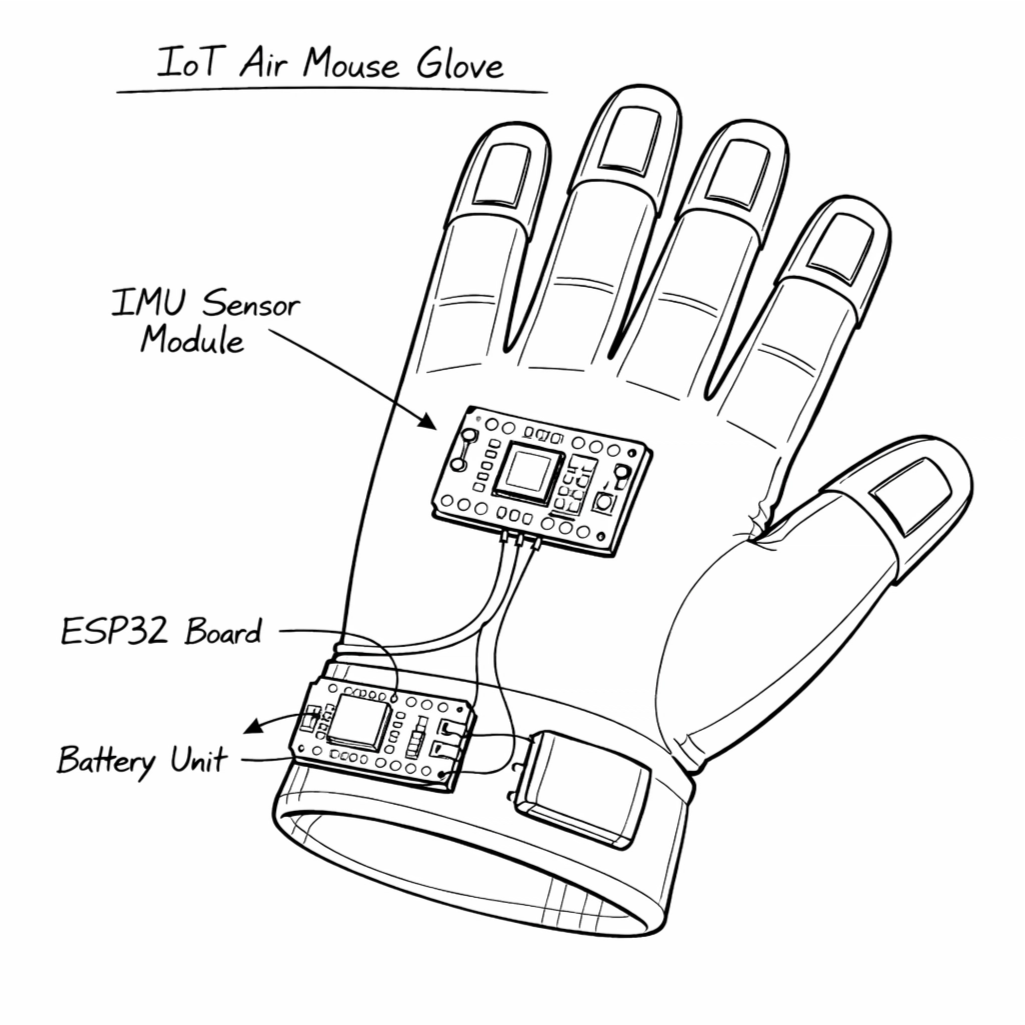
\includegraphics[width=0.5\textwidth]{img/air_mouse_glove_sketch.png}
    \caption{Conceptual Sketch of the AirGlove}
    \label{fig:sketch}
    
\end{figure}

The primary mechanism for motion tracking is centered around a high-precision Inertial Measurement Unit (IMU), such as the MPU6050 or MPU6500. These sensors integrate a three-axis accelerometer and a three-axis gyroscope to capture both linear acceleration and angular velocity. Through the use of onboard Digital Motion Processing (DMP) and sensor fusion algorithms the system can accurately determine the orientation and tilt of the hand while filtering out mechanical noise and drift. This data is then translated into cursor movement, where the gyroscope handles fine rotational adjustments and the accelerometer detects broader directional shifts. For simpler implementations or power-constrained scenarios, a standalone three-axis accelerometer like the ADXL345 can be employed to detect basic tilt-based movement, though the 6-axis IMU remains the standard for professional-grade responsiveness \cite{mummadi2018imu_glove}.


To facilitate user interaction, the glove incorporates strategically placed finger contact points and conductive pathways. These contact points, typically located on the tips of the index and middle fingers and the side of the thumb, utilize conductive fabrics or silver-plated threads to act as soft, wearable switches. When the user brings the thumb into contact with a specific finger pad, a circuit is closed, which the system interprets as a left-click, right-click, or scroll activation. This textile-based approach ensures that the glove remains flexible and comfortable for extended use, avoiding the bulk of traditional mechanical buttons. Furthermore, the integration of a dedicated sensitivity switch allows users to dynamically adjust the control gain. This hardware-level toggle enables the microcontroller to scale the sensor data in real-time, allowing the user to switch between high-sensitivity modes for rapid navigation and low-sensitivity modes for precision tasks like digital drawing or detailed selection.

The processing and communication hub of the device is the ESP32 microcontroller, chosen for its powerful dual-core architecture and integrated wireless capabilities. The ESP32 handles the real-time acquisition of sensor data via I2C or SPI interfaces, executes the gesture recognition logic, and manages the Bluetooth Low Energy (BLE) or 2.4GHz HID profile to communicate with the host computer. This allows the glove to appear as a standard wireless mouse to any operating system without requiring specialized drivers \cite{prayogi2024esp32_airmouse}.

% \begin{figure}[h]
%     \centering
%     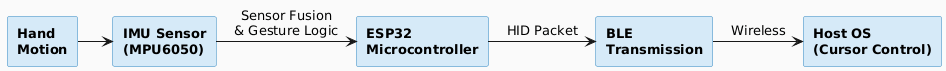
\includegraphics[width=1\textwidth]{img/flow.png}
%     \caption{Processing Flow}
%     \label{fig:processing_flow}
    
% \end{figure}

% At the system level, the glove's operation can be described as a closed sensing processing communication pipeline, illustrated in Figure \ref{fig:processing_flow}. Motion data is continuously sampled by the IMU at a configurable rate, transmitted to the ESP32, where a firmware layer applies sensor fusion and gesture classification. Valid gesture events — such as a sustained tilt beyond a defined angular threshold or a finger contact closure — are encoded into standard HID mouse report packets and transmitted via BLE to the paired host device. The host operating system processes these packets identically to any USB or Bluetooth mouse, requiring no custom drivers. This architecture ensures low latency between physical gesture and cursor response, while the modular firmware structure allows future extension to support additional gestures such as scroll, zoom, or multi-finger shortcuts.

\section{Comparative Analysis}
This section positions the proposed AirGlove prototype against existing commercial air-mouse products and relevant research prototypes. The goal is to clarify what the system already does well, where it currently falls short, and which constraints are most likely to affect real-world usability and adoption. The analysis is structured in three parts: first, a SWOT evaluation summarizes internal strengths and limitations alongside external opportunities and risks; second, a structured comparison table consolidates key differences in form factor, sensing approach, interaction capabilities, connectivity, and practical constraints; finally, a brief research and industry context highlights trends that inform realistic improvement paths for future iterations.

\subsection{SWOT Analysis}

In order to better understand the current state of midair pointing devices and wearable input technologies, existing commercial solutions and research prototypes were analyzed. The market currently includes handheld air mice, presenter remotes, and experimental glove-based input devices, which demonstrate both the practicability and the limitations of midair cursor control. Based on this analysis, a SWOT (Strengths, Weaknesses, Opportunities, Threats) evaluation was conducted to assess the proposed air mouse glove solution using ESP32 and MPU6050/MPU6500 sensors. The full comparative analysis is provided in Appendix~\ref{appendix:comparative_table}, while Table~\ref{tbl:swot} summarizes the main strengths, weaknesses, opportunities, and threats of the proposed design.


\subsection{Comparative Analysis}

As shown in Table \ref{tbl:comparative_air_mouse}, the comparative analysis highlights several important distinctions across the evaluated solutions. In terms of form factor and wearability, the proposed glove shares the wearable category with experimental concepts such as Ion and Bellcos, as well as research prototypes, but differentiates itself from handheld remotes and presenter devices by eliminating the need to grip or hold any physical object.

Regarding interaction method, commercial air mice rely on tilt-based motion but offer no gesture vocabulary beyond cursor movement and button clicks, whereas the proposed design inherits gesture support (scroll, zoom, pause mode) from its research-prototype lineage \cite{cornell_airmouse_project,acm_airmouse_interface} while adding Bluetooth HID connectivity characteristic of commercial devices. With respect to sensor technology, all IMU-based solutions share the same fundamental sensing principle (gyroscope and accelerometer fusion) but differ substantially in the quality: commercial products ship with factory-tuned firmware, while the proposed prototype requires custom filter implementation. This represents both the main current weakness of the prototype and its primary long-term advantage, since the filtering strategy is fully adjustable and can be iteratively improved.

On connectivity, the proposed glove is designed to operate primarily as a native Bluetooth HID device without a USB dongle, which improves portability compared to 2.4 GHz receiver-dependent commercial remotes. A 2.4 GHz variant remains a possible extension for environments where Bluetooth is restricted or unreliable. Regarding precision and stability, the proposed design is rated as tunable, honestly reflecting the current prototype stage; commercial devices rated medium or medium--high are factory-optimised but cannot be modified, whereas the proposed glove's precision ceiling is determined by the sophistication of the algorithms applied rather than by fixed hardware constraints. 

Battery life is a dimension routinely overlooked in product-level comparisons of air mice, yet it is critically important for wearable devices intended for real-world use. Commercial devices suffer a well-documented limitation in this regard: user reviews consistently cite short operational duration as a key frustration \cite{reddit_airmouse_discussion}, and none of the handheld or experimental wearable solutions evaluated offer a transparent power management strategy. The proposed design, powered by a LiPo battery connected to the ESP32, does not resolve this issue at the prototype stage; however, its open architecture allows power consumption to be actively managed through deep-sleep modes and duty-cycling, an optimisation path unavailable in any closed commercial product.

Similarly, customisability is a differentiating factor that commercial solutions cannot offer by design. The proposed glove is unique among the evaluated solutions in being fully open: every layer of the system, from sensor calibration and gesture mapping to Bluetooth HID report descriptors, is accessible and modifiable. This is significant not only for ongoing development but also for the research and accessibility use cases the device targets, where gesture vocabularies and sensitivity profiles may need to be adapted per user or per deployment context.

Overall, the picture that emerges is nuanced. The proposed design does not yet match commercial devices in terms of polish, battery life, or out-of-box precision. However, it outperforms them in portability, wearability, customisability, and the potential ceiling of its pointing performance, advantages being only realisable through continued algorithmic development and iterative hardware refinement.

\subsection{Industry Trends and Research Context}

The proposed air mouse glove is positioned within a specific and well-defined niche: IMU-based wearable devices used as pointing and cursor-control interfaces. This section surveys relevant research and commercial developments within that niche, rather than the broader gesture recognition industry, which includes unrelated application domains such as automotive infotainment, touchscreen panels, and computer-vision systems.


\subsubsection{IMU Wearables as Pointing Devices: Research Trends}

Research interest in IMU-based wearable pointing devices has grown steadily within the HCI community. A representative recent example is \textit{MouseRing}, presented at ACM CHI~2024 \cite{acm_airmouse_interface}, which proposes an IMU ring-shaped device enabling continuous finger-based cursor control on unmodified surfaces, targeting always-available interaction in AR/VR and large-screen environments. The work explicitly identifies the same core design tension faced by the proposed glove: the need to retain the comfort and precision of conventional pointing while eliminating the physical and environmental constraints of surface-dependent devices.

Similarly, research into IMU-based assistive mouse controllers, such as the \textit{Auxilio} system, which uses a low-cost commercial IMU to enable cursor control for users with upper-limb disabilities, demonstrates that the principle of mapping IMU orientation to cursor movement is already validated in peer-reviewed HCI literature \cite{arxiv_gesture_recognition}. These works confirm that the sensing approach underlying the proposed air mouse glove is technically sound and aligned with active research directions.

\subsubsection{IMU as the Preferred Sensor Modality for Wearable Pointing}

Within the wearable pointing-device domain, IMUs have emerged as the sensor of choice due to their low power consumption, compact form factor, low cost, and independence from line-of-sight or lighting constraints, limitations that affect camera-based alternatives. Industry sources confirm that IMUs are increasingly embedded in wrist-worn and finger-worn devices for gesture input, and that their effectiveness is directly tied to the quality of the algorithms processing their output \cite{gesture_market}.

Critically, research consistently demonstrates that hardware selection alone is insufficient to determine pointing quality; the choice of sensor fusion strategy, whether Madgwick, Mahony, Complementary, or Kalman filtering, has a substantial effect on stability and drift. A 2024 study published in the \textit{International Journal of Reconfigurable and Embedded Systems} confirmed that IMU gesture classifiers using full orientation representations achieve accuracy above 99\% under embedded resource constraints, while reduced feature sets maintain accuracy above 90\% \cite{gesture_hci_research}. These findings directly support the algorithmic approach adopted in the proposed design, in which sensor fusion and calibration routines are treated as core engineering priorities rather than secondary concerns.

\subsubsection{Accessibility and the Case for Surface-Independent Input}

A recurring motivation in the IMU wearable pointing literature is accessibility: enabling computer interaction for users who cannot comfortably use a conventional mouse or touchpad. The \textit{Auxilio} project specifically targets users with upper-limb disabilities by replacing the desktop mouse with an IMU-driven interface, demonstrating that cursor mapping from body-worn inertial sensors is a clinically viable approach.

More broadly, the HCI research community has documented demand for input solutions that are portable, surface-independent, and ergonomically undemanding, which are requirements that align directly with the intended use cases of the proposed glove, namely presentation control and accessibility. The Wearable Devices and Doublepoint collaboration further illustrates that this design space is attracting commercial investment: their \textit{WowMouse} platform converts an Apple Watch into an air gesture pointing device using on-wrist IMU data and embedded algorithms, demonstrating commercial viability for the same underlying concept.

\subsubsection{Future Directions: Miniaturisation and On-Device AI}

Two related trends are likely to influence the next generation of IMU-based pointing devices. The first is continued miniaturisation of IMU hardware. New “smart IMU” solutions, such as the Bosch BHI360, can run gesture-related algorithms directly on the sensor, which supports smaller designs and lower power consumption.

For the proposed glove, this means that the current ESP32 + MPU6050/6500 setup, while suitable for prototyping, could later be replaced with a more integrated module that offers better drift behaviour and reduced energy use. The second trend is progress in TinyML, where machine-learning models are designed to run efficiently on microcontrollers. Recent work shows that on-device gesture classification can fit within the memory and compute limits of platforms similar to the ESP32 \cite{arxiv_airmouse_future}. This suggests a possible future upgrade path rather than a current project goal: the present system will rely on rule-based calibration, while a later iteration could add lightweight trained classifiers to improve robustness across different users and reduce sensitivity to unintended movements, all while keeping processing on-device.
\section{Target Audience \& Stakeholders}

While the previous sections established the technical and ergonomic landscape of wearable input devices, the viability of a glove-based air mouse depends entirely on its alignment with specific human needs and market realities. This section identifies the priority audiences and stakeholder-relevant user profiles for the proposed system, moving beyond general utility to define concrete adoption segments.

\subsection{Target Audience Segments and Adoption Rationale}

The broadest segment is the population of everyday technology users who are already comfortable with computers and Bluetooth peripherals but seek better ergonomics, mobility, or interaction novelty than conventional desk-bound mice. For this group, value is primarily practical: they need stable cursor response, low-friction pairing, and battery endurance sufficient for routine sessions in flexible contexts such as standing desks, couch/bed use, and ad hoc workspaces where a flat surface is inconvenient. This segment is strategically important because it provides the largest baseline adoption pool and the fastest path to real-world usage feedback.

The market scale for this segment is substantial. Recent market estimates place global PC users at approximately 1.86 billion, with continued annual growth in the low single-digit range~\cite{explodingtopics_pc_users_2024}. Even conservative conversion rates in such a base represent a meaningful opportunity for alternative input peripherals. Ergonomic burden within general computer users further supports this relevance: a Swedish population-oriented report indicates that musculoskeletal discomfort during computer work is common even among users without formal diagnosis, reinforcing that demand for alternatives is not limited to clinical populations~\cite{arbetsmiljoverket_workrelated_disorders_2024}. Occupational burden data from labor surveillance similarly indicate that repetitive-trauma exposure remains a major source of upper-limb injury and illness in modern work~\cite{bls_iif_2024}.

A second, high-priority segment is users with physical disability, reduced dexterity, or repetitive strain injury (RSI), including users affected by carpal tunnel syndrome (CTS), arthritis-related pain, post-stroke weakness, or persistent wrist/forearm overuse. For this segment, the glove is not merely a convenience accessory; it is an accessibility intervention. Surface-free interaction removes wrist-on-desk pressure, and threshold-based gesture logic can be tuned for reduced grip strength or constrained range of motion. This is especially relevant when commercial assistive alternatives are costly or offer limited customization.

Clinical and occupational evidence supports this priority. U.S. injury surveillance reports large annual burdens of work-related musculoskeletal injury and repetitive-trauma outcomes~\cite{bls_iif_2024,cdc_ergonomics_2024}. In the computer-using population specifically, prior evidence already included in this dissertation documents elevated CTS prevalence and strong exposure links in mouse-intensive work~\cite{dale2013cts,andersen2003mouse,thomsen2008mouse}. Broader accessibility evidence also supports the segment's strategic importance: people with disability remain under-served in digital access and device ownership, which implies a continuing need for adaptable and affordable interaction alternatives~\cite{perrin2021disabilitytech,duplaga2017disability}. From a product perspective, this segment also imposes the most stringent design constraints, making it a strong anchor for requirement quality.

A third high-value segment is presenters and educators, particularly in hybrid teaching and meeting environments where users need to move freely while maintaining control over slides, pointer movement, media playback, and annotation. The core behavioral pattern already exists in this market through wireless clickers and presenter remotes. The glove proposition is therefore not behavioral replacement, but functional expansion: one wearable controller for both navigation and full cursor interaction. Market analyses report sustained growth in wireless presentation-controller categories and related interactive classroom ecosystems, indicating stable demand for presentation mobility tools~\cite{wiredclicker_market_2024,verifiedmarketreports_clicker_2023}.

A fourth segment is gamers and VR/AR enthusiasts, where perceived immersion and expressive control can motivate early experimentation with unconventional input hardware. This segment is performance-sensitive and therefore acts as a stress test for latency, fusion stability, and gesture reliability. Global gaming participation and PC gaming market size remain extremely large, while enthusiast communities are often receptive to customizable open-source hardware and firmware workflows~\cite{newzoo_gaming_2024,steam_concurrent_2025}. For this audience, the glove concept is attractive only if end-to-end delay and aiming stability approach competitive usability thresholds.

Taken together, these segments define a clear prioritization strategy. Everyday users provide scale, disability/RSI users provide the strongest social and accessibility impact, presenters/educators provide immediate workflow fit, and gaming communities provide performance-driven refinement pressure. This multi-segment structure improves deployment realism by balancing market size, inclusion value, and technical rigor.

\subsection{Representative Use Cases and Persona-Driven Requirements}

Use-case analysis translates segment-level assumptions into concrete interaction scenarios. In rehabilitation-oriented home or clinic settings, a user recovering from stroke may have partial hand movement but difficulty gripping or sliding a traditional mouse. In this scenario, low-amplitude wrist rotation combined with simple finger gestures can restore core digital independence for browsing, communication, and form completion. In education settings, a lecturer can move between board and audience while controlling slides and cursor without returning to a desk device. In advanced productivity or gaming contexts, users can combine one-hand gestural pointing with keyboard shortcuts for command-dense workflows.

To operationalize these scenarios, this chapter introduces a representative persona: \textbf{Marco R.}, a 34-year-old freelance graphic designer based in Valencia who works remotely and spends 6--10 hours daily on design tools. Marco has a history of CTS-related pain, has already tested vertical and trackball devices with only partial relief, and requires high cursor precision for visual editing tasks. His central constraint is not basic computer literacy but sustained usability under pain and fatigue. This profile is strategically useful because it combines high precision demand, prolonged exposure, moderate technical confidence, and strong motivation to adopt alternatives if setup friction is low.

Marco's requirement profile is practical and measurable: zero wrist-to-surface contact, precision sufficient for design software, adjustable sensitivity without firmware editing, battery life above one extended session, and reliable Bluetooth pairing on mainstream desktop platforms. His pain points include recurring daily discomfort with conventional mice, high prices for specialized assistive devices, and inability to self-maintain code-level settings during active work. In product terms, this implies that usability depends as much on onboarding and stability as on raw sensing quality.

Figure~\ref{fig:ch5_persona_profile} summarizes this persona using normalized usage and constraint indicators derived from the provided profile. The figure is intended as a requirement communication artifact: it visually prioritizes what must be optimized first during prototype maturation.

\begin{figure}[H]
  \centering
  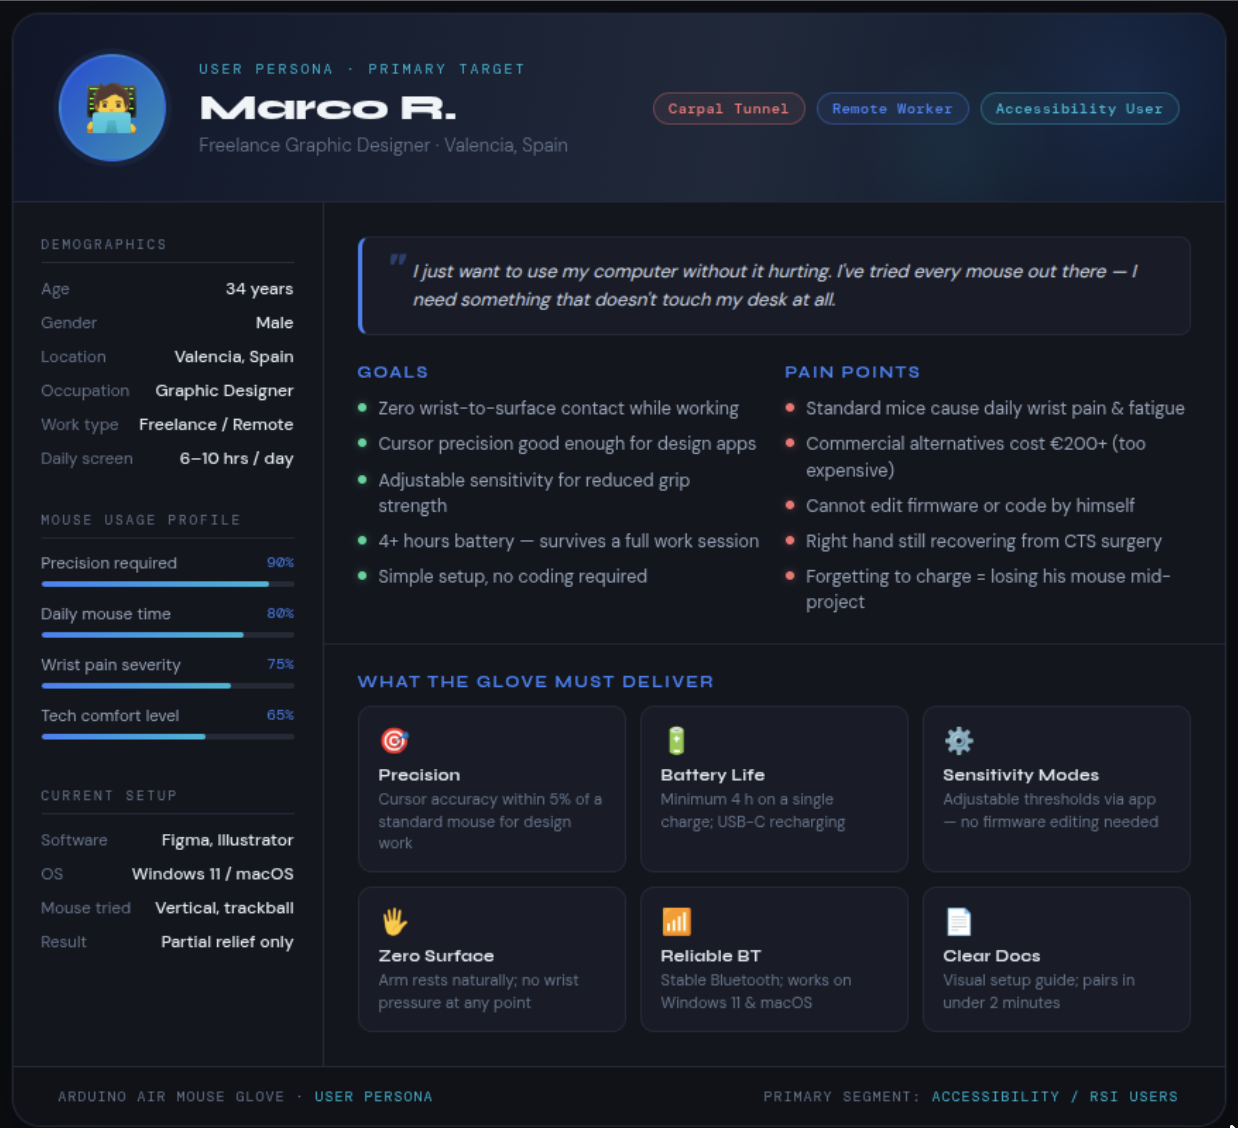
\includegraphics[width=0.6\linewidth]{img/1.png}
  \caption{User Persona Profile for a High-Precision Remote Worker in CTS Recovery}
  \label{fig:ch5_persona_profile}
\end{figure}

Interpreted together, the use cases and persona data provide direct engineering direction. Cursor behavior must remain stable during low-amplitude motion, click actions must avoid accidental displacement, pairing and reconnection must be predictable, and energy management must cover uninterrupted work sessions. These are not optional quality features: they are minimum viability conditions for the most meaningful target users.

\subsection{User Validation \& Statistical Analysis}

The following analysis based on $N=100$ respondents validates the core hypothesis: there is a clear demand for a wearable, gesture-based peripheral, particularly for specialized professional and ergonomic use cases.

% --- DISCOMFORT ANALYSIS ---
\subsubsection{Ergonomic Pain Points}
\begin{figure}[H]
    \centering
    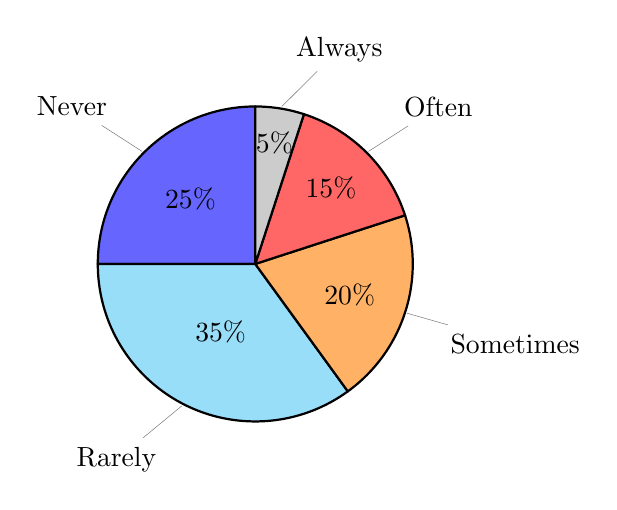
\begin{tikzpicture}
        \pie[rotate=90, text=pin, radius=2.0, color={blue!60, cyan!40, orange!60, red!60, gray!40}]{
            25/Never, 35/Rarely, 20/Sometimes, 15/Often, 5/Always
        }
    \end{tikzpicture}
    \caption{Frequency of Mouse-Related Discomfort}
\end{figure}

\textbf{Analysis:} Over \textbf{40\% of users} report experiencing discomfort "Sometimes" to "Always," while only 25\% report "Never." This distribution confirms that wrist-strain risk is not a marginal issue but a mainstream usability constraint. The ergonomic value proposition should therefore be framed as \textit{pain prevention and fatigue reduction}, not only as interaction novelty. In practical terms, this supports prioritising low-force click gestures, drift-resistant pointer behaviour during micro-movements, and calibration modes for users with reduced range of motion.

% --- USE CASE ANALYSIS ---
\subsubsection{Market Segmentation and Use Cases}

\begin{figure}[H]
    \centering
    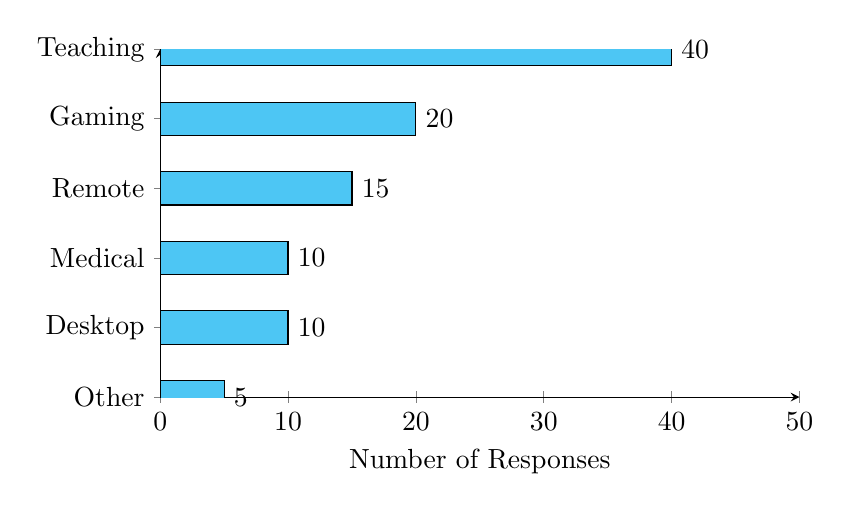
\begin{tikzpicture}
        \begin{axis}[
            xbar, xmin=0, xmax=50, width=0.8\textwidth, height=6cm,
            xlabel={Number of Responses},
            symbolic y coords={{Other}, {Desktop}, {Medical}, {Remote}, {Gaming}, {Teaching}},
            ytick=data, nodes near coords, nodes near coords align={horizontal},
            axis x line=bottom, axis y line=left, bar width=12pt
        ]
            \addplot[fill=cyan!70] coordinates {(40,{Teaching}) (20,{Gaming}) (15,{Remote}) (10,{Medical}) (10,{Desktop}) (5,{Other})};
        \end{axis}
    \end{tikzpicture}
    \caption{Primary Use Case Validation}
\end{figure}

The data identifies \textbf{Presentations and Teaching (40\%)} as the primary entry market, followed by Gaming (20\%) and Remote Work (15\%). This indicates that \textit{mobility-centric contexts} dominate early adoption intent: users value standing movement, room-scale interaction, and cursor control away from a fixed desk. Strategically, this supports a phased go-to-market model: first optimise presenter-grade reliability (slide navigation, stable cursor, rapid reconnect), then expand toward precision-demand segments such as design-heavy remote work and gaming. The chart therefore justifies a "Pro-Presenter first, precision expansion second" product trajectory rather than immediate mass-market desktop replacement.



% --- BARRIERS & ADOPTION ---
\subsubsection{Adoption Likelihood vs. Technical Barriers}
\begin{figure}[H]
    \centering
    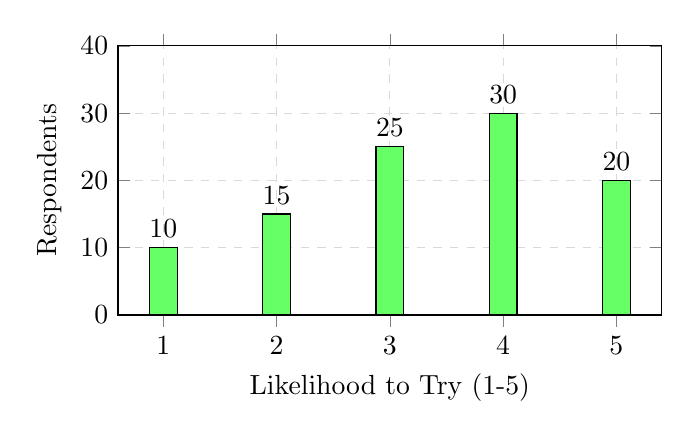
\begin{tikzpicture}
        \begin{axis}[
            ybar, ymin=0, ymax=40, width=0.7\textwidth, height=5cm,
            ylabel={Respondents}, xlabel={Likelihood to Try (1-5)},
            xtick=data, symbolic x coords={1, 2, 3, 4, 5},
            nodes near coords, grid=major, grid style={dashed, gray!30}
        ]
            \addplot[fill=green!60] coordinates {(1,10) (2,15) (3,25) (4,30) (5,20)};
        \end{axis}
    \end{tikzpicture}
    \caption{Consumer Interest Distribution}
\end{figure}

\textbf{Analysis:} With \textbf{50\% of respondents} scoring 4 or 5, baseline willingness to trial is strong; however, the central adoption signal is \textit{conditional enthusiasm}. Users are interested, but conversion depends on two gatekeepers: cost (30\%) and perceived precision (25\%). This implies that technical maturity and affordability must progress together. From an engineering perspective, the prototype should transition from exploratory sensing to a higher-stability IMU pipeline with improved filtering, repeatable calibration, and quantifiable jitter control. From a product perspective, bill-of-material choices should be evaluated against a target entry price band so that performance gains are not negated by cost-driven drop-off.





\subsection{Stakeholders}

Beyond direct users, the present work involves stakeholders who influence adoption, validation, and long-term viability. Population-level digital access disparities reinforce this broader relevance: adults with disabilities report lower computer ownership (62\% versus 81\%) and higher rates of never going online (15\% versus 5\%) than adults without disabilities~\cite{perrin2021disabilitytech}. Similar disparities are reported in non-US settings, including substantially lower internet participation among respondents with disabilities in Poland~\cite{duplaga2017disability}. At organisational level, the stakeholder case is also economic: musculoskeletal disorders have been associated with major direct and indirect occupational costs~\cite{nrc2001msd}, while WHO/ILO estimates indicate sustained growth in work-related musculoskeletal burden over time~\cite{whoilo2021wrmsd}. Appendix Table~\ref{tbl:stakeholders_appendix} summarises the main groups, their interests, and the evidence supporting their relevance.
\begin{figure}[H]
\centering
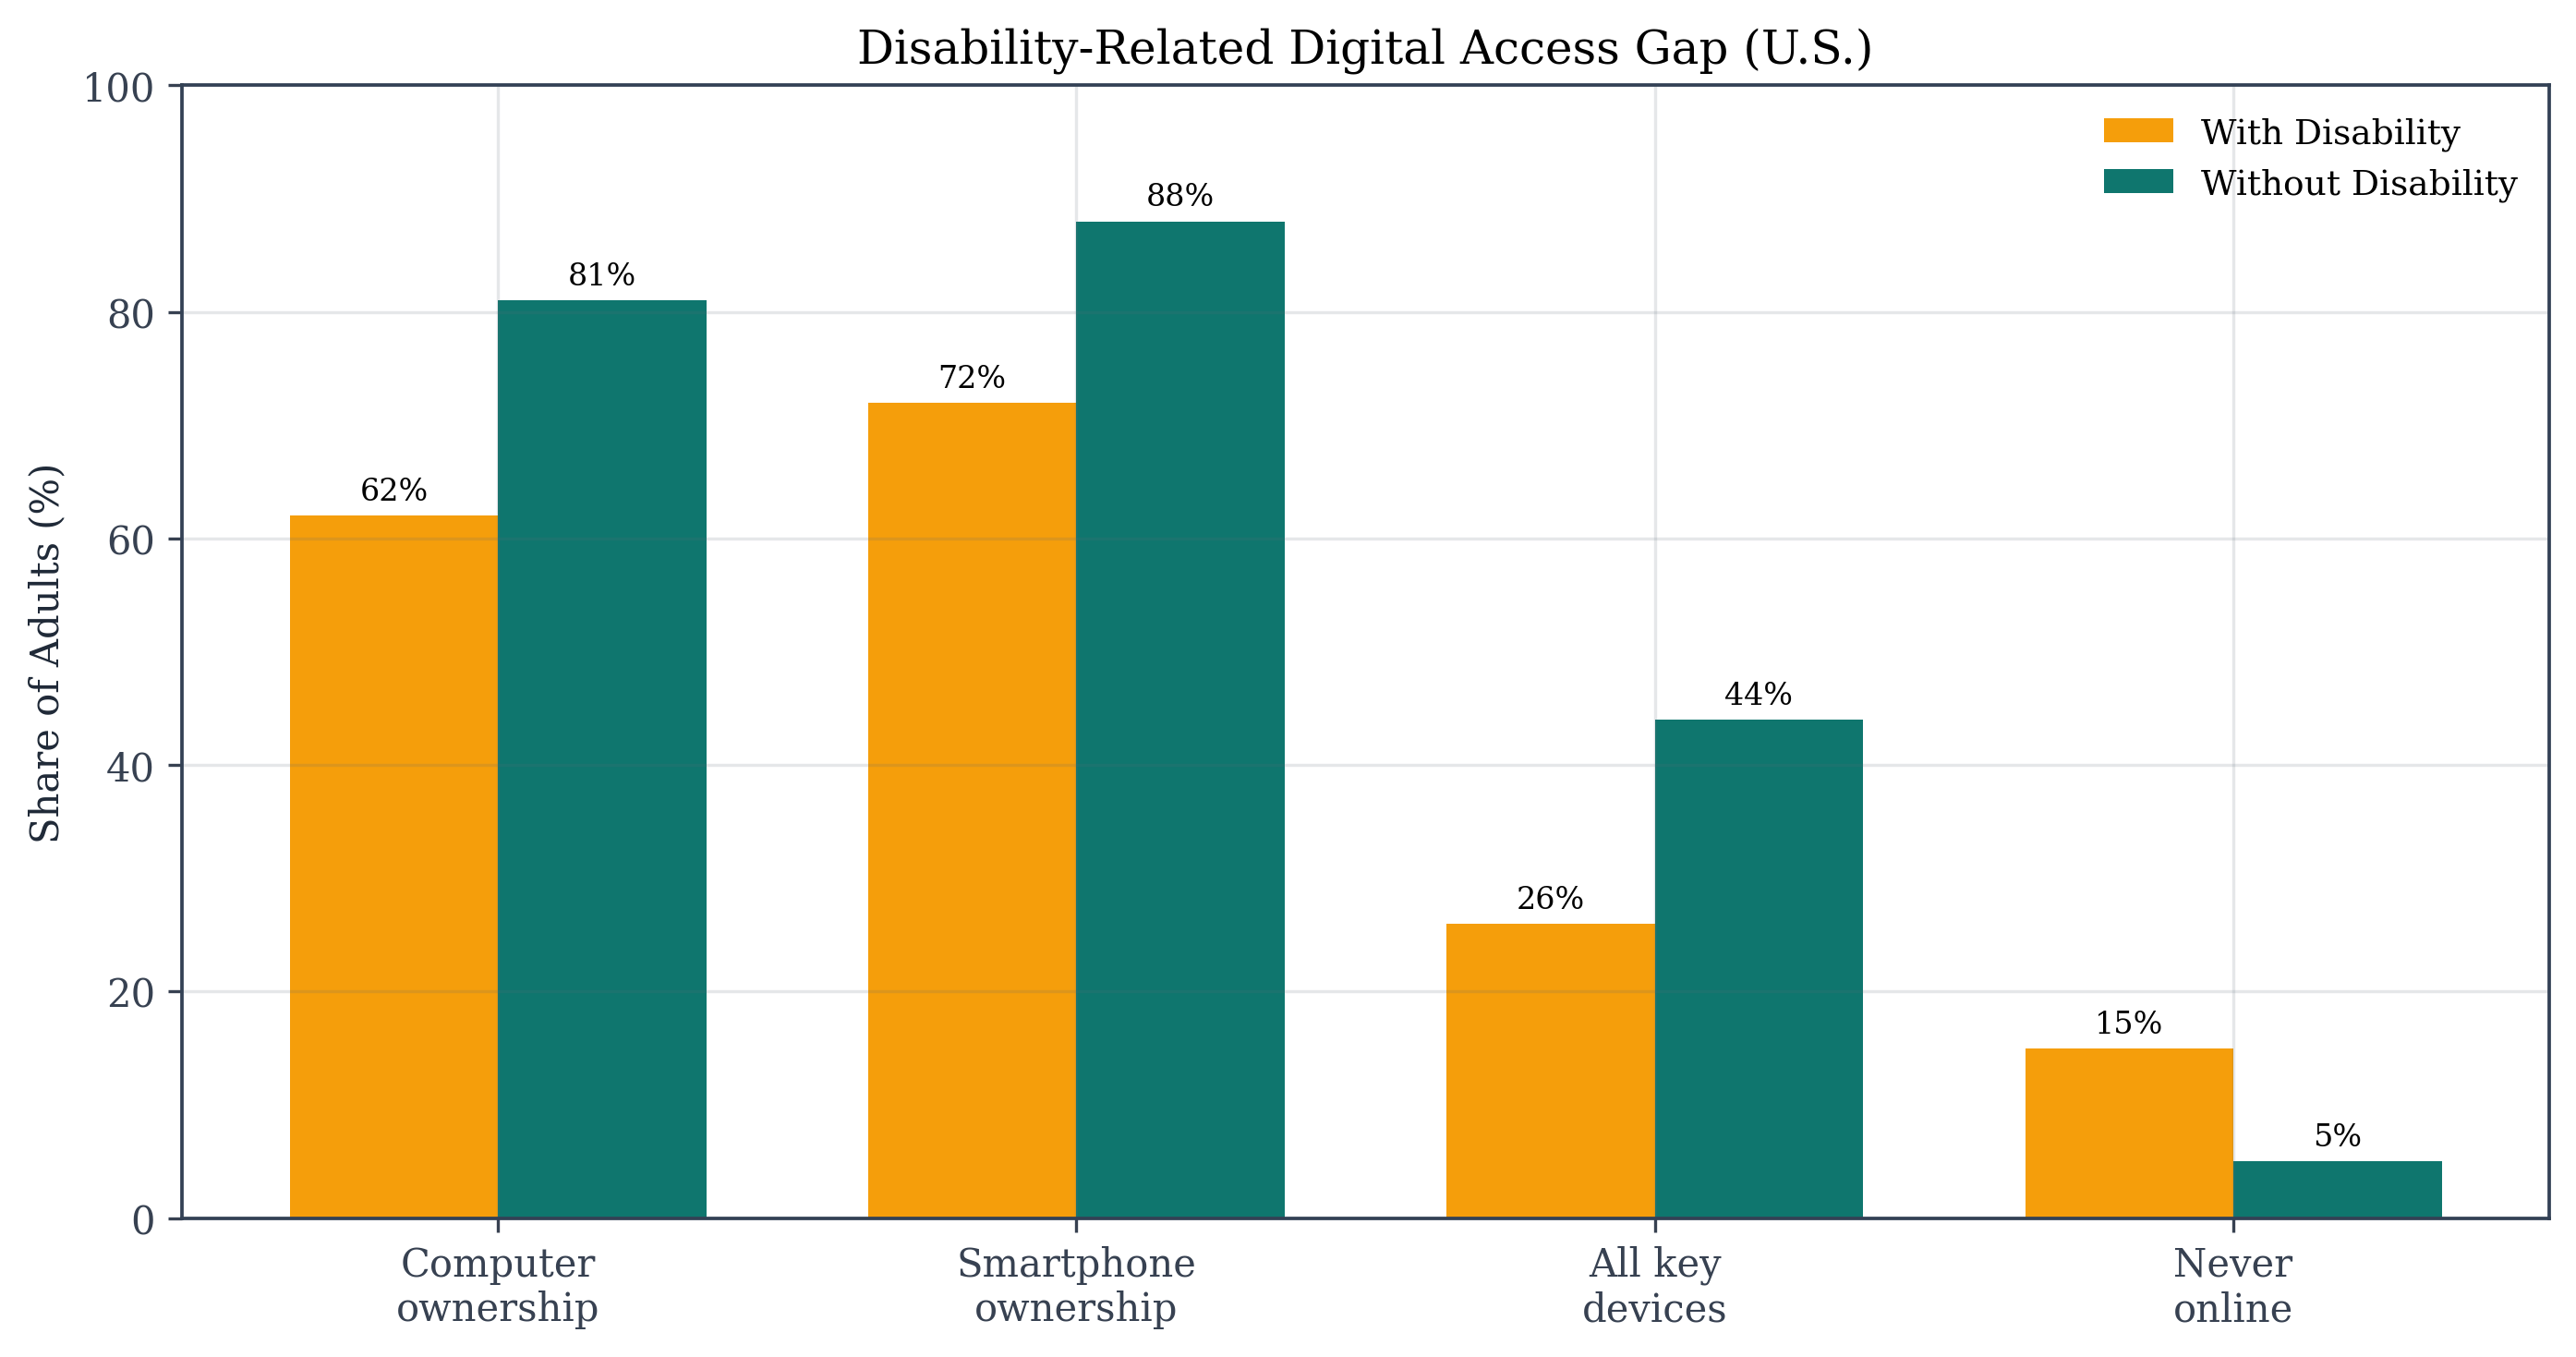
\includegraphics[width=0.75\linewidth]{img/ch5_disability_digital_divide.png}
\caption{Disability-Related Digital Access Gap in U.S. Survey Data}
\label{fig:digital_divide_stakeholder}
\end{figure}
Figure~\ref{fig:digital_divide_stakeholder} visualises the digital-access asymmetry that motivates stakeholder involvement beyond direct end users, particularly for institutions responsible for equitable deployment.



For stakeholder analysis, this pattern indicates that accessibility constraints are not isolated edge cases but population-level participation constraints. Consequently, institutional stakeholders are relevant not only for procurement and deployment but also for inclusion outcomes.

The detailed stakeholder matrix is provided in Appendix Table~\ref{tbl:stakeholders_appendix}.



The table operationalises stakeholder prioritisation by linking each group to a concrete validation signal, which supports transparent evaluation criteria in later chapters.

\subsection{Design Implications, Stakeholder Fit, and Validation Priorities}

The target-audience analysis creates a concrete bridge between user diversity and implementation planning. For everyday users, success depends on simplicity and perceived reliability: fast setup, robust Bluetooth behavior, and low-maintenance operation. For disability and RSI populations, success depends on tunable sensitivity, low-force interaction, and repeatable control under motor variability. For presenters and educators, success depends on mobility without control interruption. For gamers and enthusiasts, success depends on latency discipline and response consistency under high interaction frequency. 

These requirements also map cleanly to stakeholder interests discussed in earlier chapters. Accessibility practitioners and rehabilitation professionals can evaluate personalization benefit. Educational institutions can evaluate deployment in teaching environments. Employers and occupational-health stakeholders can evaluate ergonomic sustainability in high-exposure computer workflows. Open-source contributors can iterate sensing and interaction logic using transparent firmware pathways. This alignment is important because it increases the probability of adoption beyond single-user prototypes.





\chapter{REQUIREMENTS}

This chapter defines the system requirements for AirGlove, a wearable air-mouse designed for surface-independent computer interaction. The requirements are organized into functional and non-functional groups so implementation decisions, prototype validation, and future improvements can be tracked consistently.

\section{Functional Requirements}

Functional requirements define the mandatory behaviors AirGlove must provide for complete and usable mouse interaction in real-world contexts such as presentations, remote work, and accessibility-oriented usage. Each requirement is written as a verifiable system behavior consistent with the proposed architecture in this report.

\begin{itemize}
    \item \textbf{FR 1. Device initialization and ready state.} After power-on, the system shall initialize the IMU sensor module, finger-contact input channels, and Bluetooth HID service in a single startup sequence. The device shall enter an operational state without requiring custom host-side software.

    \item \textbf{FR 2. Bluetooth pairing and automatic reconnection.} The system shall support first-time pairing with a target host and store bonding information for future sessions. On temporary disconnection, the device shall attempt reconnection automatically to reduce workflow interruptions.

    \item \textbf{FR 3. Mid-air cursor motion control.} The system shall transform inertial hand motion into continuous two-dimensional cursor movement on the host device. This function shall use a processing pipeline that combines sensor filtering, motion mapping, and runtime gain control.

    \item \textbf{FR 4. Click event generation through finger contact.} The system shall detect predefined finger-contact patterns and map them to standard mouse click actions (left and right click). Input logic shall include debouncing or equivalent protection to prevent frequent accidental clicks during normal cursor movement.

    \item \textbf{FR 5. Scroll interaction mode.} The system shall provide a dedicated mechanism for vertical scrolling through either explicit mode switching or dedicated contact logic. Scroll behavior shall remain distinct from pointer movement to reduce unintended mixed actions.

    \item \textbf{FR 6. Clutch and hand repositioning support.} The system shall provide a clutch mechanism that temporarily suspends cursor displacement while preserving session context. This function shall allow users to reset hand posture or neutral orientation without introducing uncontrolled pointer jumps.

    \item \textbf{FR 7. Adjustable sensitivity profiles.} The system shall offer at least two selectable sensitivity modes to support both precision tasks and rapid navigation. Switching between profiles shall be available during active use without firmware reprogramming or host-side utilities.

    \item \textbf{FR 8. User calibration workflow.} The system shall include a repeatable calibration process for neutral orientation, motion scaling, and baseline drift compensation. Calibration shall be user-triggerable so different users can adapt control behavior to their own movement patterns.

    \item \textbf{FR 9. Fault-safe runtime behavior.} The system shall detect abnormal runtime states such as unstable sensor values, transmission interruptions, or temporary packet loss. In such states, the device shall maintain controlled behavior (for example, suppressing erratic cursor output) and recover normal operation without requiring full restart.

    \item \textbf{FR 10. Host-side compatibility through HID standard.} The system shall expose input reports using a standard Bluetooth HID mouse profile. Paired desktop operating systems shall recognize AirGlove as a conventional pointing device without additional drivers or middleware installation.
\end{itemize}

\subsection{Functional Prioritization Plan}

To support incremental development and validation, functional requirements are prioritized in three implementation phases.

\begin{itemize}
    \item \textbf{Phase I (MVP interaction core).} FR 1--FR 4: startup, pairing, cursor movement, and finger-contact click input.
    \item \textbf{Phase II (usability expansion).} FR 5--FR 8: scroll mode, clutch support, sensitivity switching, and user calibration.
    \item \textbf{Phase III (robust deployment).} FR 9--FR 10: fault-safe behavior and cross-platform host compatibility.
\end{itemize}
    
\section{Non-Functional Requirements}





In addition to the functional behavior of the system, the AirGlove project must satisfy several non-functional requirements that define the quality, reliability, and usability of the proposed solution. Non-functional requirements describe how the system should operate rather than what operations it performs. Since the project aims to develop a wearable air mouse that allows users to control a computer cursor through hand movements and finger gestures, aspects such as responsiveness, comfort, stability, and reliability become essential for practical use.

First, the system must ensure a high level of usability. The interaction model should be intuitive so that users can easily understand how to control the cursor and perform click actions through natural hand movements and finger contacts. The learning curve should be minimal, allowing a new user to begin interacting with the device after a short familiarization period.

Another important requirement is ergonomics and comfort. Because the system is implemented as a glove that is worn directly on the hand, it must be lightweight and should not restrict natural hand motion. The device should allow users to perform movements comfortably during extended periods of use without causing fatigue or discomfort. Materials and component placement must therefore support natural wrist and finger mobility.

Responsiveness is also a critical requirement. The system must process sensor data and transmit cursor movements with minimal delay so that the interaction feels smooth and natural. Any noticeable latency between hand movement and cursor response could negatively affect user experience and reduce the effectiveness of the device.

Accuracy and stability of cursor control must also be maintained. The system should interpret hand movements in a stable manner and reduce unwanted cursor drift, jitter, or accidental click events. Proper filtering and processing of sensor data are necessary to ensure that small involuntary movements do not significantly affect pointer precision.

The system must also demonstrate reliable operation. The glove should maintain stable communication with the connected computer and should function consistently throughout an interaction session. Unexpected disconnections, incorrect gesture recognition, or system freezes must be minimized in order to ensure dependable usage.

Wireless connectivity is another essential requirement. The AirGlove device must communicate with the target computer through a wireless interface such as Bluetooth. The pairing process should be simple and the connection must remain stable during normal operation without requiring complex configuration steps from the user.

Portability is also an important design objective. The system should be compact and easy to transport so that it can be used in various environments such as classrooms, presentations, or office settings where a traditional mouse may be inconvenient. The prototype must therefore maintain a small form factor while integrating all necessary components.

Energy efficiency must also be considered during the design of the system. Since the device is intended to operate as a wearable electronic system, it should consume power efficiently in order to support battery-powered operation. The device should be capable of functioning for a reasonable duration without frequent recharging.

Safety is another essential requirement. All electronic components and wiring must be integrated safely so that the device can be worn directly on the hand without risk of overheating, electrical issues, or physical discomfort. The design must avoid exposed conductors and sharp edges that could affect the user.

Finally, the system should be designed with maintainability and extensibility in mind. The architecture should allow future improvements such as adding new gesture types, improving motion processing algorithms, or integrating additional sensors. A modular design approach will simplify debugging, calibration, and future upgrades of the prototype.

By fulfilling these non-functional requirements, the AirGlove system will provide not only the expected functionality of cursor control through hand gestures, but also a practical, reliable, and comfortable interaction device that can serve as a viable alternative to conventional computer input peripherals.



% \section{High-Level System Architecture}

% \begin{figure}[H]
%     \centering
%     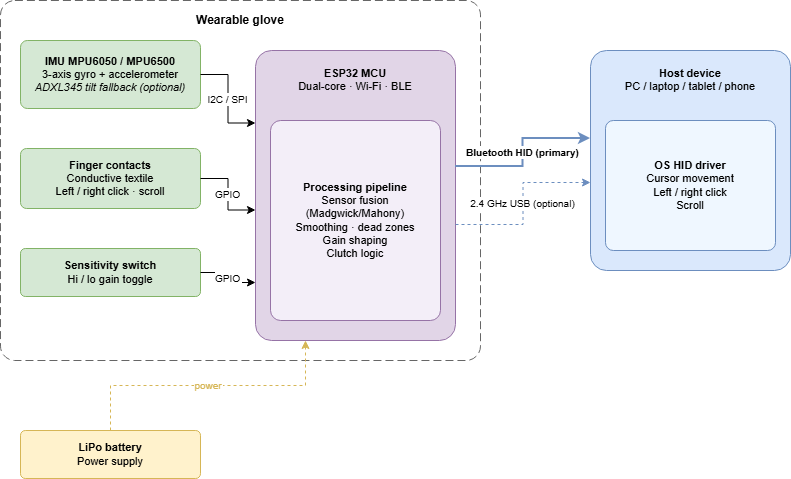
\includegraphics[width=\textwidth]{img/architectural_final.drawio.png}
%     \caption{High-level IoT architecture of the AirGlove system}
%     \label{fig:high_level_iot_architecture}
% \end{figure}
\chapter{SYSTEM DESIGN}

The architecture of the air mouse glove, illustrated in Figure \ref{fig:system-design}, is structured around three functional layers: the sensor input layer, the processing and communication core, and the host device interface. Together, these layers form a complete wireless human-computer interaction system embedded within a wearable glove form factor.

\begin{figure}[hb]
    \centering
    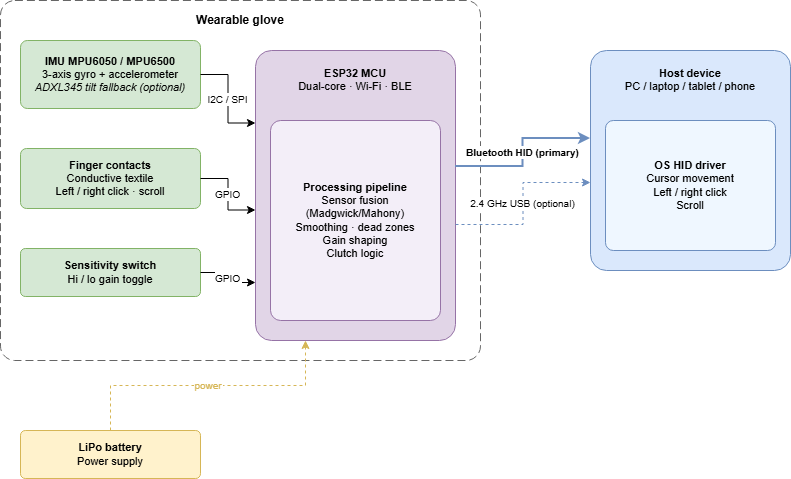
\includegraphics[width=0.9\textwidth]{img/architectural_final.drawio.png}
    \caption{System Architecture}
    \label{fig:system-design}
\end{figure}

\section*{Sensor Input Layer}

The primary motion sensing component is the \textbf{MPU-6050} (or its lower-cost variant, the MPU-6500), a six-axis Inertial Measurement Unit (IMU) that combines a 3-axis gyroscope and a 3-axis accelerometer on a single chip. The gyroscope measures angular velocity across the roll, pitch, and yaw axes, while the accelerometer captures linear acceleration and gravitational orientation. Together, these two data streams allow the system to reconstruct the full spatial orientation of the user's hand in real time. For scenarios requiring enhanced tilt accuracy or redundancy, an \textbf{ADXL345} accelerometer can be incorporated as an optional fallback device. Both the MPU-6050 and the ADXL345 communicate with the ESP32 microcontroller over the \textbf{I\textsuperscript{2}C or SPI} serial interfaces, which allow multiple devices to share the same communication bus with minimal wiring overhead.

User input beyond motion is handled by two additional components connected via \textbf{GPIO} pins on the ESP32. The \textbf{finger contact sensors}, implemented using conductive textile integrated into the glove's fingertips, detect discrete touch events and are mapped to left click, right click, and scroll actions, directly mirroring the button layout of a conventional mouse. A dedicated \textbf{sensitivity switch} provides a hardware-level \textit{hi/lo gain toggle}, enabling the user to switch between a high-sensitivity mode (suitable for fine cursor control) and a low-sensitivity mode (better suited for broad movements across large displays), without requiring any software interaction.

\section*{Processing and Communication Core}

The central processing unit of the system is the \textbf{ESP32 microcontroller}, a dual-core, 32-bit system-on-chip that integrates both \textbf{Wi-Fi} and \textbf{Bluetooth Low Energy (BLE)} radios. Its dual-core architecture allows sensor acquisition and data transmission to run concurrently without blocking each other, which is critical for maintaining low-latency cursor response.

Raw IMU data is passed through a multi-stage \textbf{processing pipeline} before being transmitted. The first stage applies a \textbf{sensor fusion algorithm}, specifically either the \textit{Madgwick} or \textit{Mahony} filter, which mathematically combines gyroscope and accelerometer readings to produce a stable quaternion-based orientation estimate. These complementary filters are computationally efficient and well-suited for embedded systems, correcting gyroscope drift over time using accelerometer gravity references. The fused orientation data is then processed through several additional stages: \textbf{smoothing filters} reduce high-frequency noise caused by natural hand tremors; \textbf{dead zones} suppress very small, unintentional movements below a configurable threshold so the cursor remains stationary when the hand is at rest; \textbf{gain shaping} applies a non-linear transfer function to map hand movement magnitude to cursor displacement speed, allowing slow movements to produce fine precision while fast movements yield rapid cursor travel; and \textbf{clutch logic} provides a mechanism to temporarily suspend cursor movement, enabling the user to reposition their hand without unintended cursor drift.

\section*{Host Device Interface}

Once processed, the orientation and button data is transmitted to the host device primarily via \textbf{Bluetooth HID} (Human Interface Device profile). This standard protocol allows the glove to present itself to any host operating system as a native wireless pointing device, requiring no proprietary drivers or software installation on PCs, laptops, tablets, or smartphones. As an optional alternative, a \textbf{2.4 GHz USB dongle} connection is also supported, which can offer lower latency in environments with Bluetooth interference.

On the host side, the operating system's built-in \textbf{HID driver} interprets the incoming data packets and translates them directly into standard \textbf{cursor movement}, \textbf{left/right click}, and \textbf{scroll} events, identical in behavior to those generated by a conventional mouse.

\section*{Power Supply}

The entire system is powered by a \textbf{LiPo} (Lithium Polymer) battery integrated into the glove. LiPo cells are well suited for this application due to their high energy density, lightweight form factor, and flat, flexible packaging that conforms naturally to wearable enclosures. The battery supplies power to both the ESP32 and all connected sensors through an onboard power regulation circuit.

\section{FR Air Glove --- UML and Architecture Diagrams}

\subsection{Overview}

Based on the analyzed implementation, \textbf{FR Air Glove} is an ESP32-based wearable BLE HID mouse. The system reads hand motion from an MPU6050 IMU and capacitive touch input from ESP32 touch pads. This input is processed by driver modules, service modules, FreeRTOS tasks, and finally converted into BLE HID mouse reports sent to a paired host device.

The diagrams in this section describe the project from different viewpoints: user functionality, high-level architecture, runtime activities, and sequence interactions between the main software modules. Each diagram is based on the real code structure and uses the actual module or function names where necessary.

\subsection{UML Use Case Diagram}

\begin{figure}[H]
    \centering
   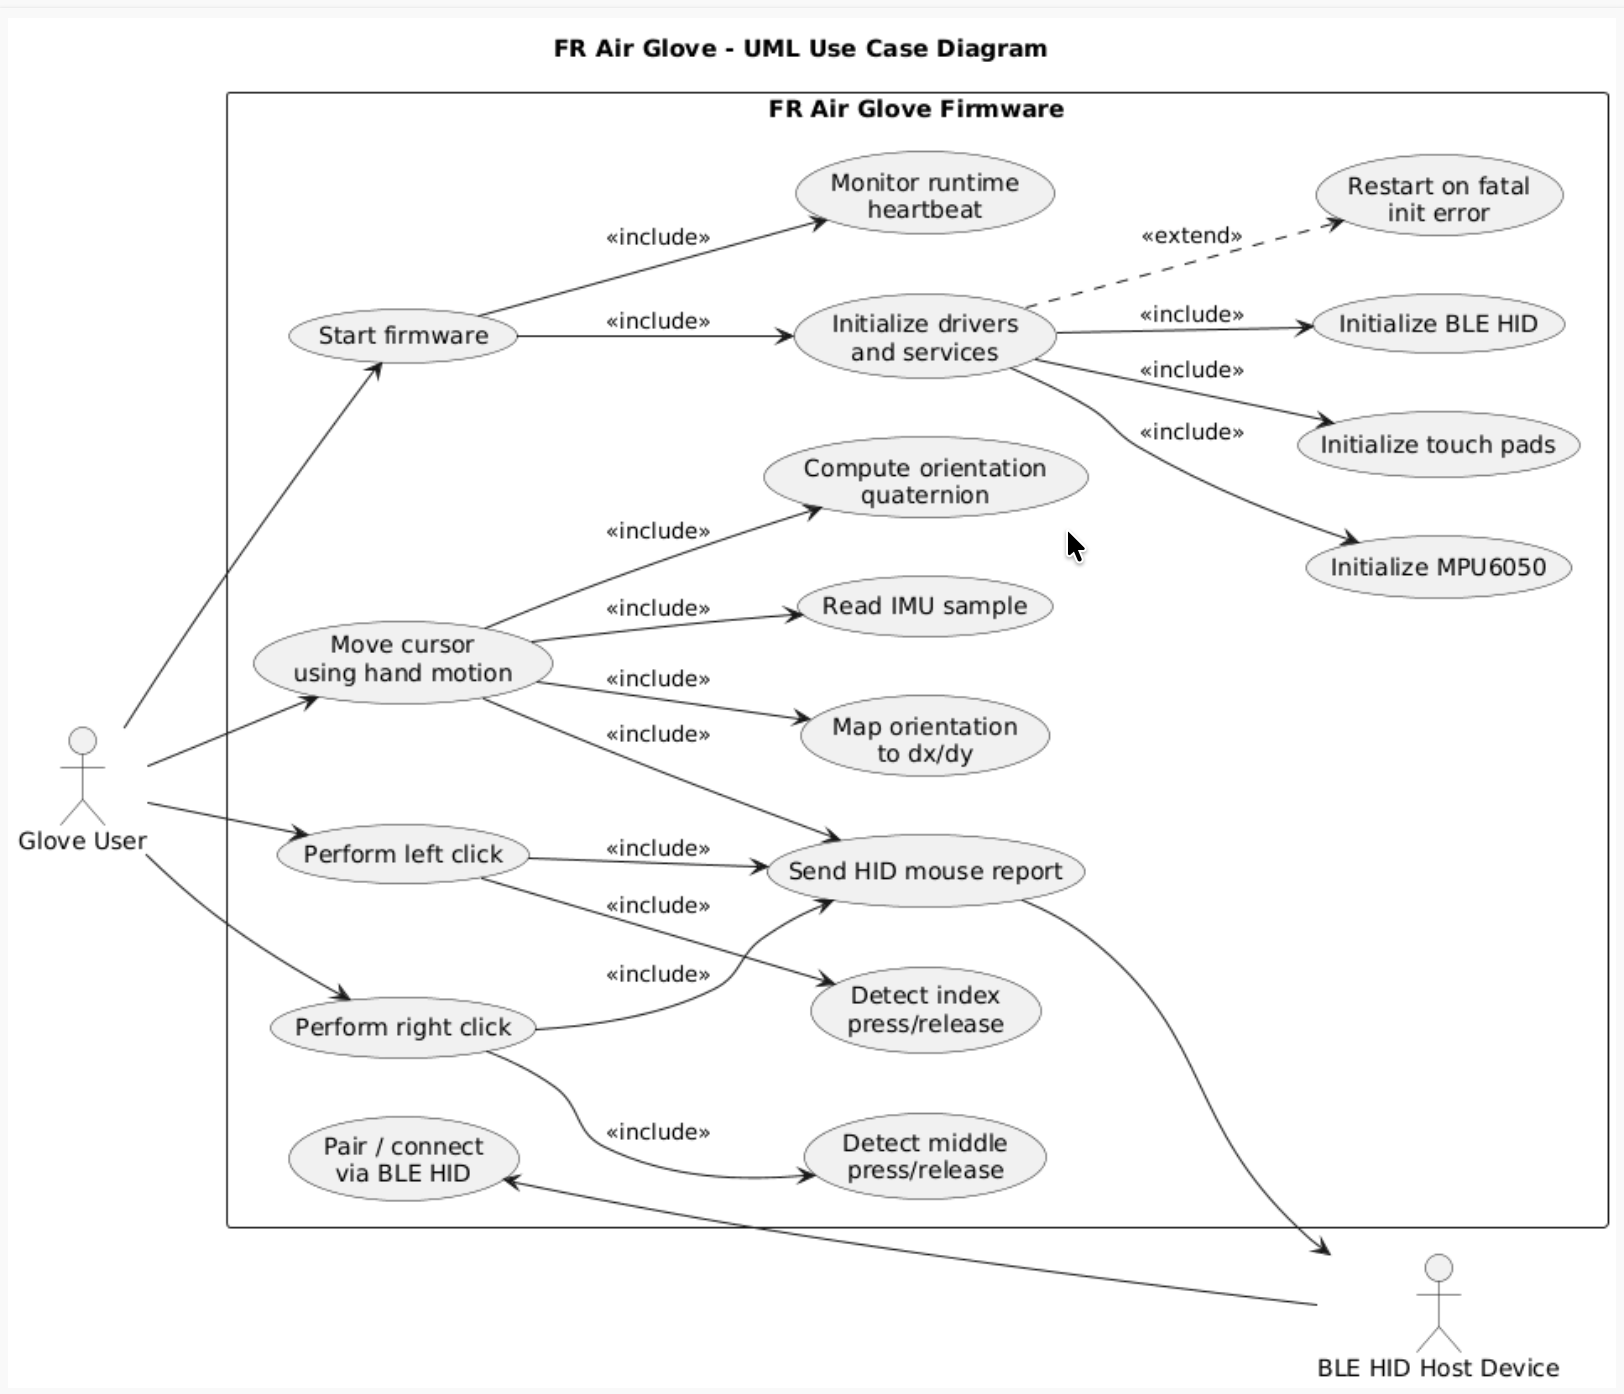
\includegraphics[width=0.5\textwidth]{img/use-case.png}
    \caption{FR Air Glove UML Use Case Diagram}
    \label{fig:fr-air-glove-use-case}
\end{figure}

The use case diagram presents the FR Air Glove system from the external user perspective. The main actor is the \textbf{Glove User}, who interacts with the device by powering it on, moving the hand, and touching specific capacitive pads. These actions are translated into mouse functions such as cursor movement, left click, and right click. The second actor is the \textbf{BLE HID Host Device}, which represents a computer, tablet, or phone that receives the HID mouse input through Bluetooth.

The system boundary represents the firmware running on the ESP32. Inside this boundary are the main functions supported by the system: starting the firmware, initializing drivers and services, pairing through BLE HID, reading IMU data, calculating orientation, mapping motion to cursor movement, detecting touch press/release actions, and sending HID mouse reports.

This diagram is useful because it gives a general overview of what the system does before explaining how the internal modules work. It also separates user-level functionality from implementation details.

Code support examples:
\begin{itemize}
    \item Firmware startup begins in \texttt{setup()}, which calls \texttt{app\_controller\_start()}.
    \item Initialization is supported by \texttt{dd\_mpu6050\_init()}, \texttt{dd\_touch\_init()}, and \texttt{dd\_ble\_hid\_init()}.
    \item Cursor movement is supported by \texttt{dd\_mpu6050\_read()}, \texttt{srv\_fusion\_update()}, and \texttt{srv\_motion\_update()}.
    \item Touch clicking is supported by \texttt{srv\_input\_process()} and the button mapping inside the application task.
\end{itemize}

\subsection{High-Level Architecture Diagram}

\begin{figure}[H]
    \centering
    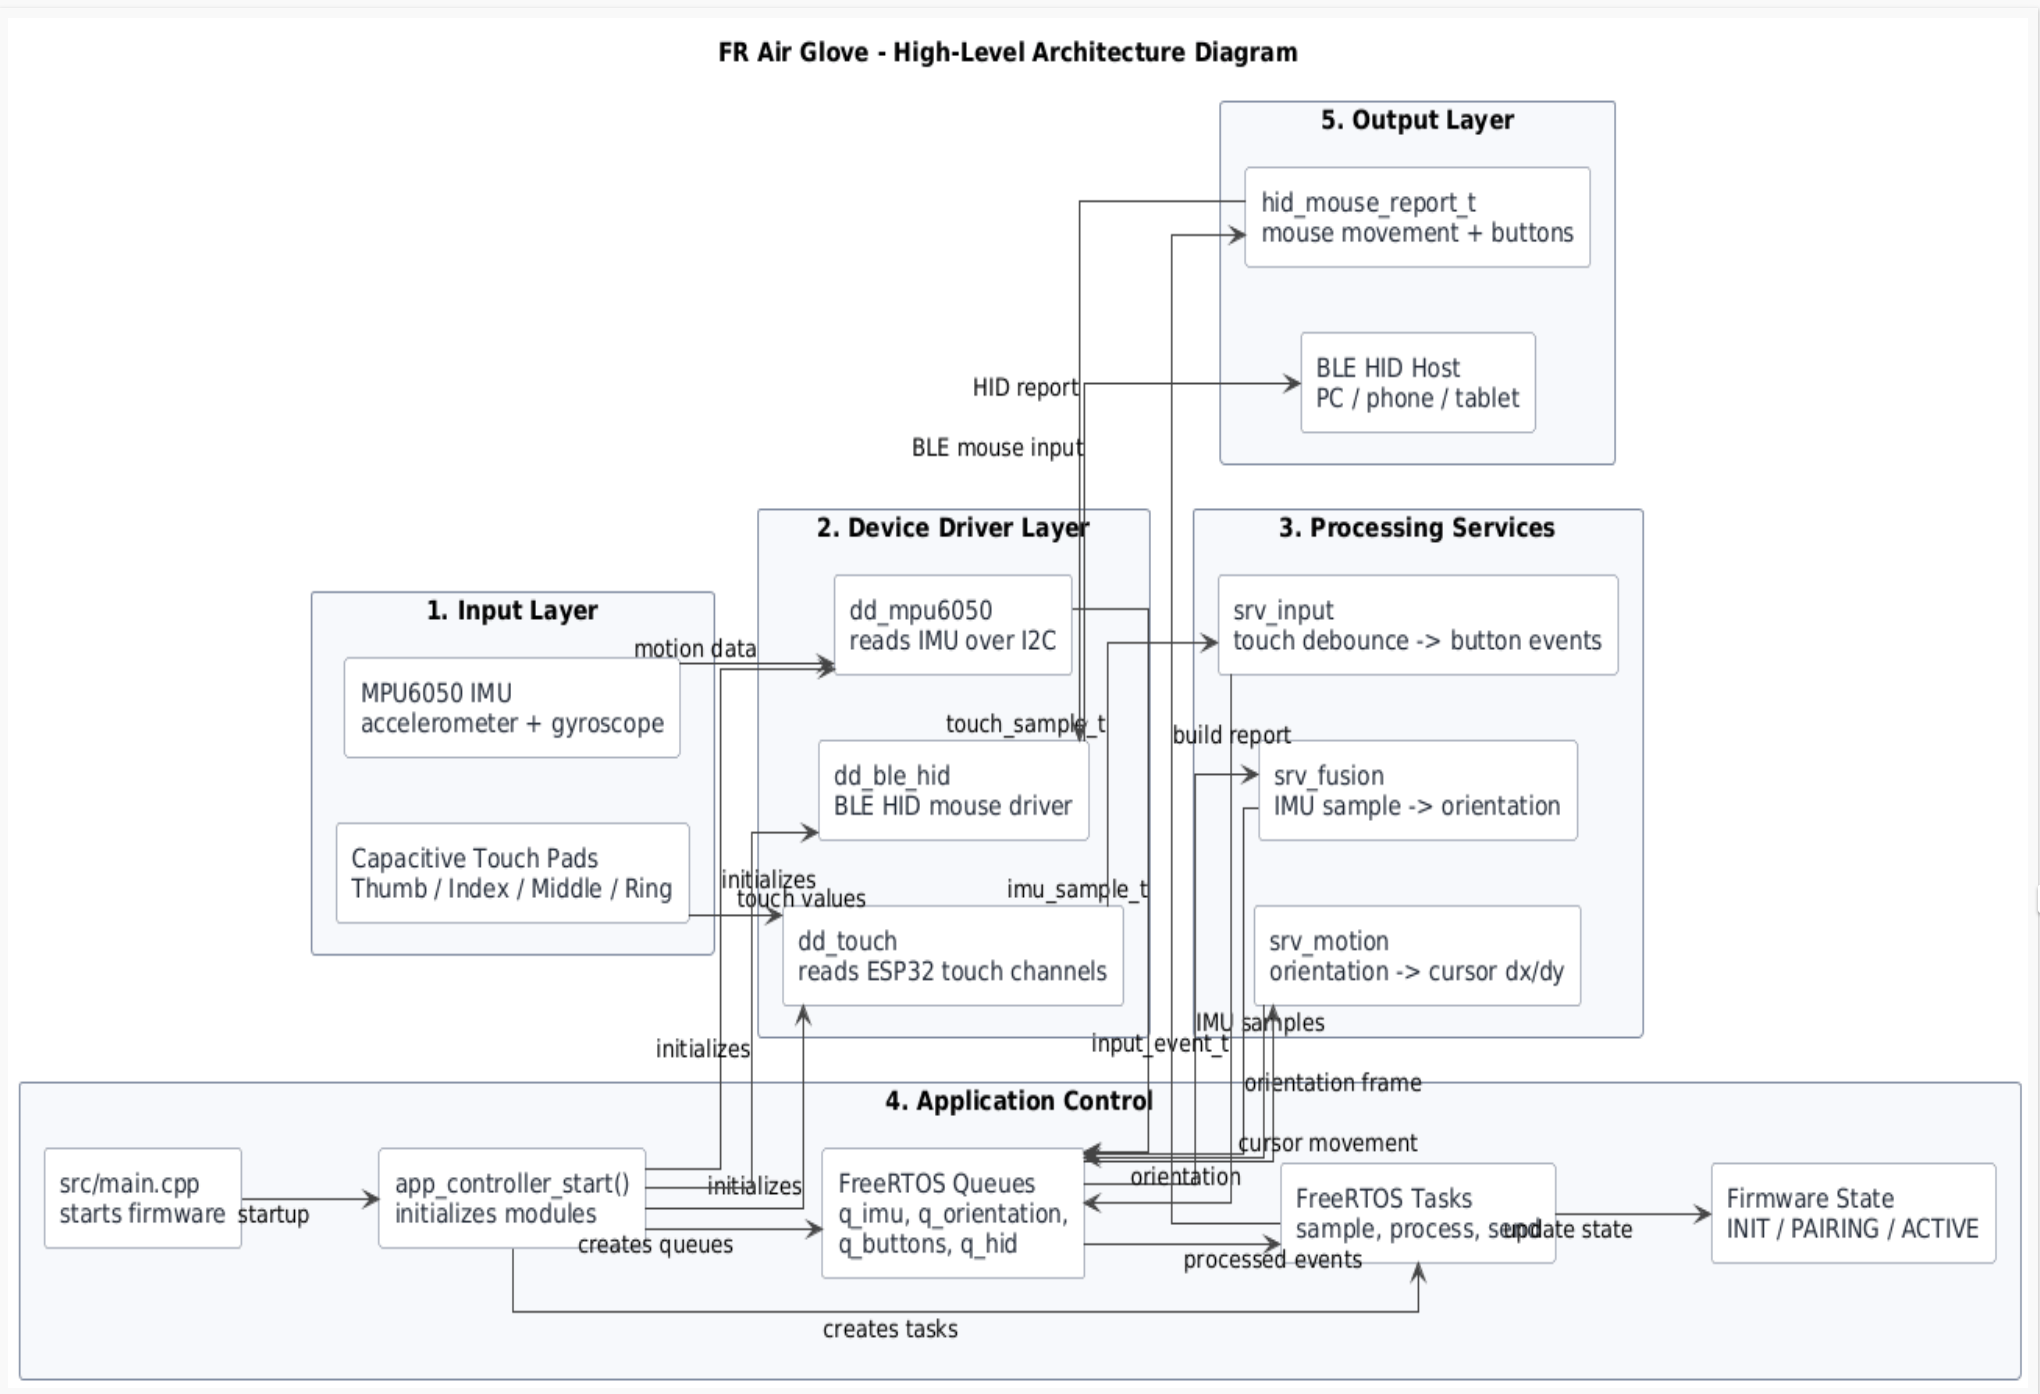
\includegraphics[width=0.8\textwidth]{img/h-l.png}
    \caption{FR Air Glove High-Level Architecture Diagram}
    \label{fig:fr-air-glove-high-level-architecture}
\end{figure}

The high-level architecture diagram shows the system as a set of logical layers. The first layer is the input layer, where the MPU6050 IMU provides movement data and the capacitive touch pads provide button input. The second layer is the device driver layer, which contains hardware-specific modules responsible for reading sensors and handling BLE HID communication.

The processing services layer transforms raw data into meaningful control data. The fusion service estimates glove orientation, the motion service converts orientation changes into cursor movement, and the input service filters touch readings into stable button events. The application control layer coordinates the system using FreeRTOS tasks and queues. Finally, the output layer contains the HID report structure and the external BLE HID host.

This architecture is important because it shows that the firmware is modular. Hardware access, processing logic, runtime control, and communication are separated into different responsibilities. This makes the project easier to understand, test, and extend.

Code support examples:
\begin{itemize}
    \item The driver layer is represented by \texttt{dd\_mpu6050}, \texttt{dd\_touch}, and \texttt{dd\_ble\_hid}.
    \item The processing layer is represented by \texttt{srv\_fusion}, \texttt{srv\_motion}, and \texttt{srv\_input}.
    \item The application layer is started through \texttt{app\_controller\_start()}.
    \item The final output is represented by \texttt{hid\_mouse\_report\_t} and sent using \texttt{dd\_ble\_hid\_send()}.
\end{itemize}

\subsection{Activity Diagrams}

The main activity diagram was divided into four smaller diagrams because the firmware contains several parallel FreeRTOS-based behaviours. Splitting the activity model makes each process easier to understand and avoids creating one large unreadable diagram.

\subsubsection{System Initialization Activity}

\begin{figure}[H]
    \centering
    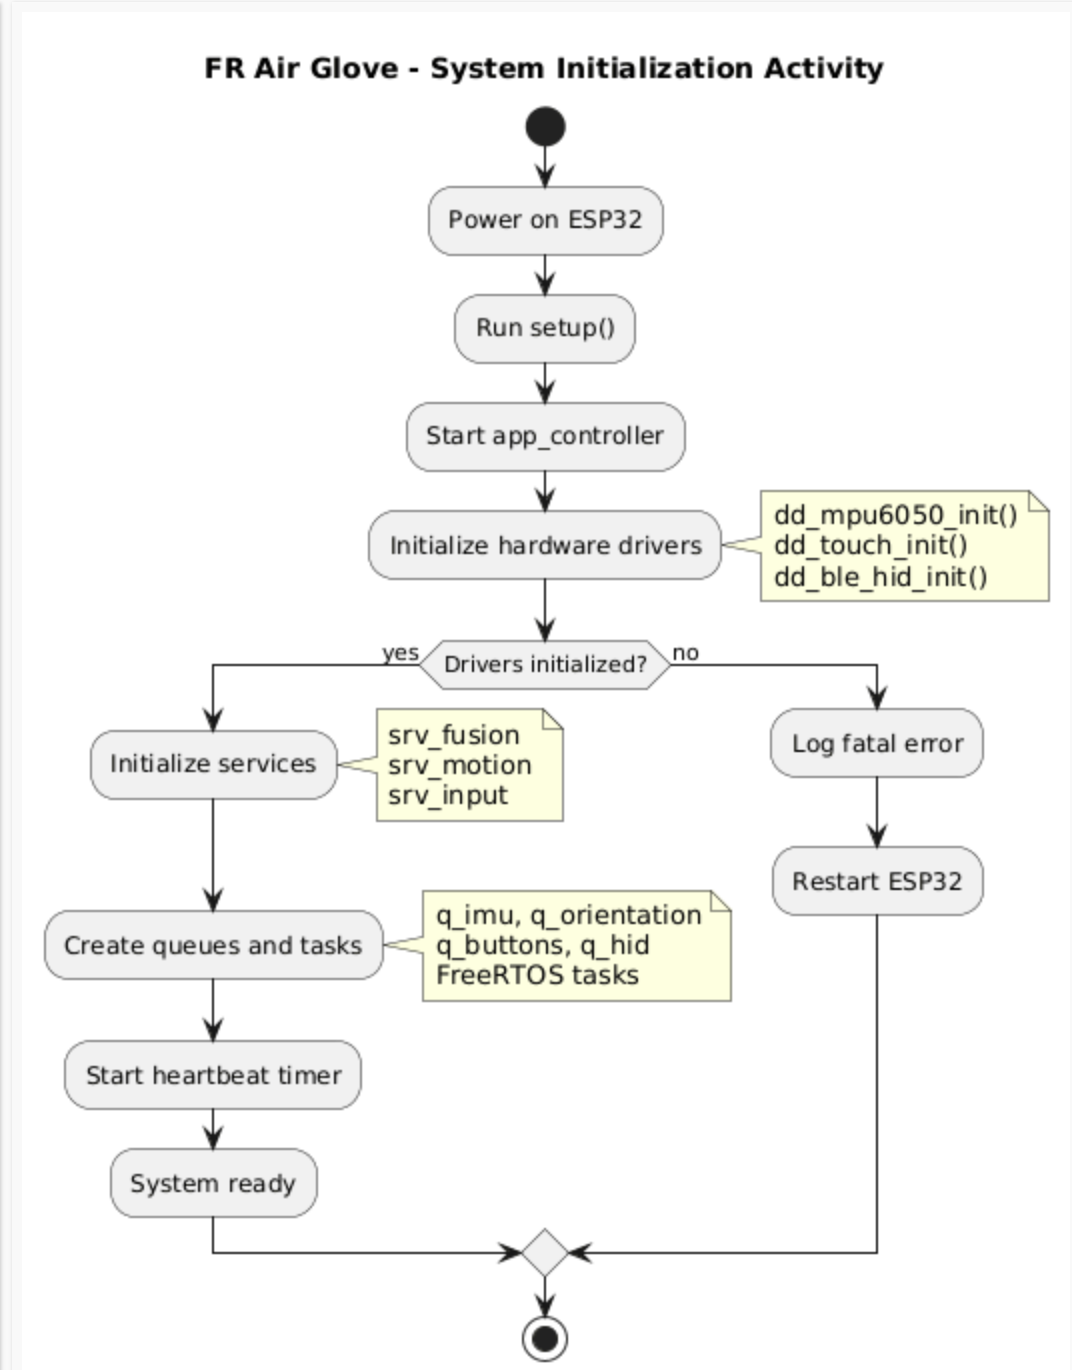
\includegraphics[width=0.5\textwidth]{img/a1.png}
    \caption{FR Air Glove System Initialization Activity Diagram}
    \label{fig:fr-air-glove-activity-initialization}
\end{figure}

The system initialization activity diagram describes how the firmware starts after the ESP32 is powered on. The process begins with the Arduino \texttt{setup()} function, which starts the application controller. The controller initializes the required hardware drivers, including the MPU6050 driver, the touch driver, and the BLE HID driver.

If driver initialization succeeds, the firmware continues by initializing the processing services. These services are responsible for sensor fusion, motion calculation, and touch input filtering. After that, the application creates FreeRTOS queues and tasks. The queues are used to transfer IMU samples, orientation data, button events, and HID reports between tasks. Finally, the heartbeat timer is started and the system becomes ready for runtime operation.

If initialization fails, the firmware follows an error path. It logs a fatal error and restarts the ESP32. This is important in embedded systems because the device should not continue running when essential hardware or communication modules are not available.

Code support examples:
\begin{itemize}
    \item Startup begins in \texttt{setup()} and continues with \texttt{app\_controller\_start()}.
    \item Hardware initialization uses \texttt{dd\_mpu6050\_init()}, \texttt{dd\_touch\_init()}, and \texttt{dd\_ble\_hid\_init()}.
    \item Service initialization uses \texttt{srv\_fusion\_init()}, \texttt{srv\_motion\_init()}, and \texttt{srv\_input\_init()}.
    \item Fatal initialization errors are handled by restarting the ESP32.
\end{itemize}

\subsubsection{IMU Motion Processing Activity}

\begin{figure}[H]
    \centering
    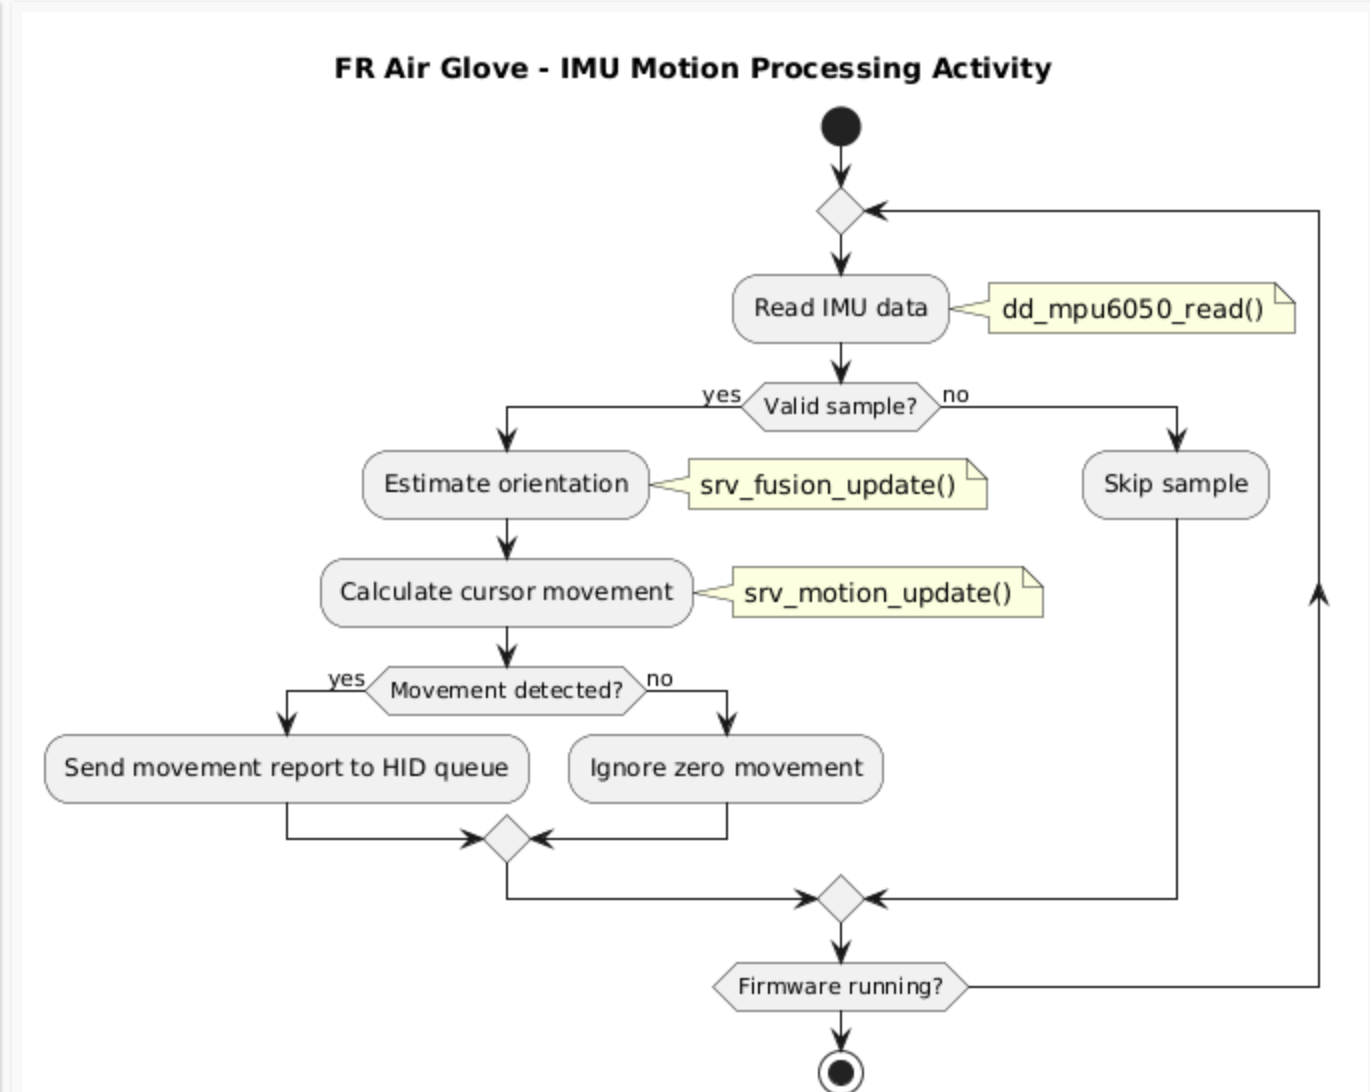
\includegraphics[width=0.5\textwidth]{img/a2.png}
    \caption{FR Air Glove IMU Motion Processing Activity Diagram}
    \label{fig:fr-air-glove-activity-imu}
\end{figure}

The IMU motion processing activity diagram explains how hand movement becomes cursor movement. The process starts by reading data from the MPU6050 IMU. If the sample is valid, the system estimates the glove orientation using the sensor fusion service. Then the motion service calculates cursor movement values from the orientation changes.

The decision point ``Movement detected?'' prevents unnecessary HID reports from being produced when there is no meaningful cursor movement. If movement is detected, a movement report is sent to the HID queue. If no movement is detected, the sample is ignored. If the IMU sample is invalid, the firmware skips the current sample and continues running.

This diagram is useful because it shows the transformation from physical hand motion to mouse cursor movement. It also shows that the firmware does not directly send every raw sensor value to the host. Instead, the data is filtered and converted into a proper HID mouse movement report.

Code support examples:
\begin{itemize}
    \item IMU data is read using \texttt{dd\_mpu6050\_read()}.
    \item Orientation estimation is performed by \texttt{srv\_fusion\_update()}.
    \item Cursor movement is calculated by \texttt{srv\_motion\_update()}.
    \item Movement results are sent as HID reports through the HID queue.
\end{itemize}

\subsubsection{Touch Button Processing Activity}

\begin{figure}[H]
    \centering
    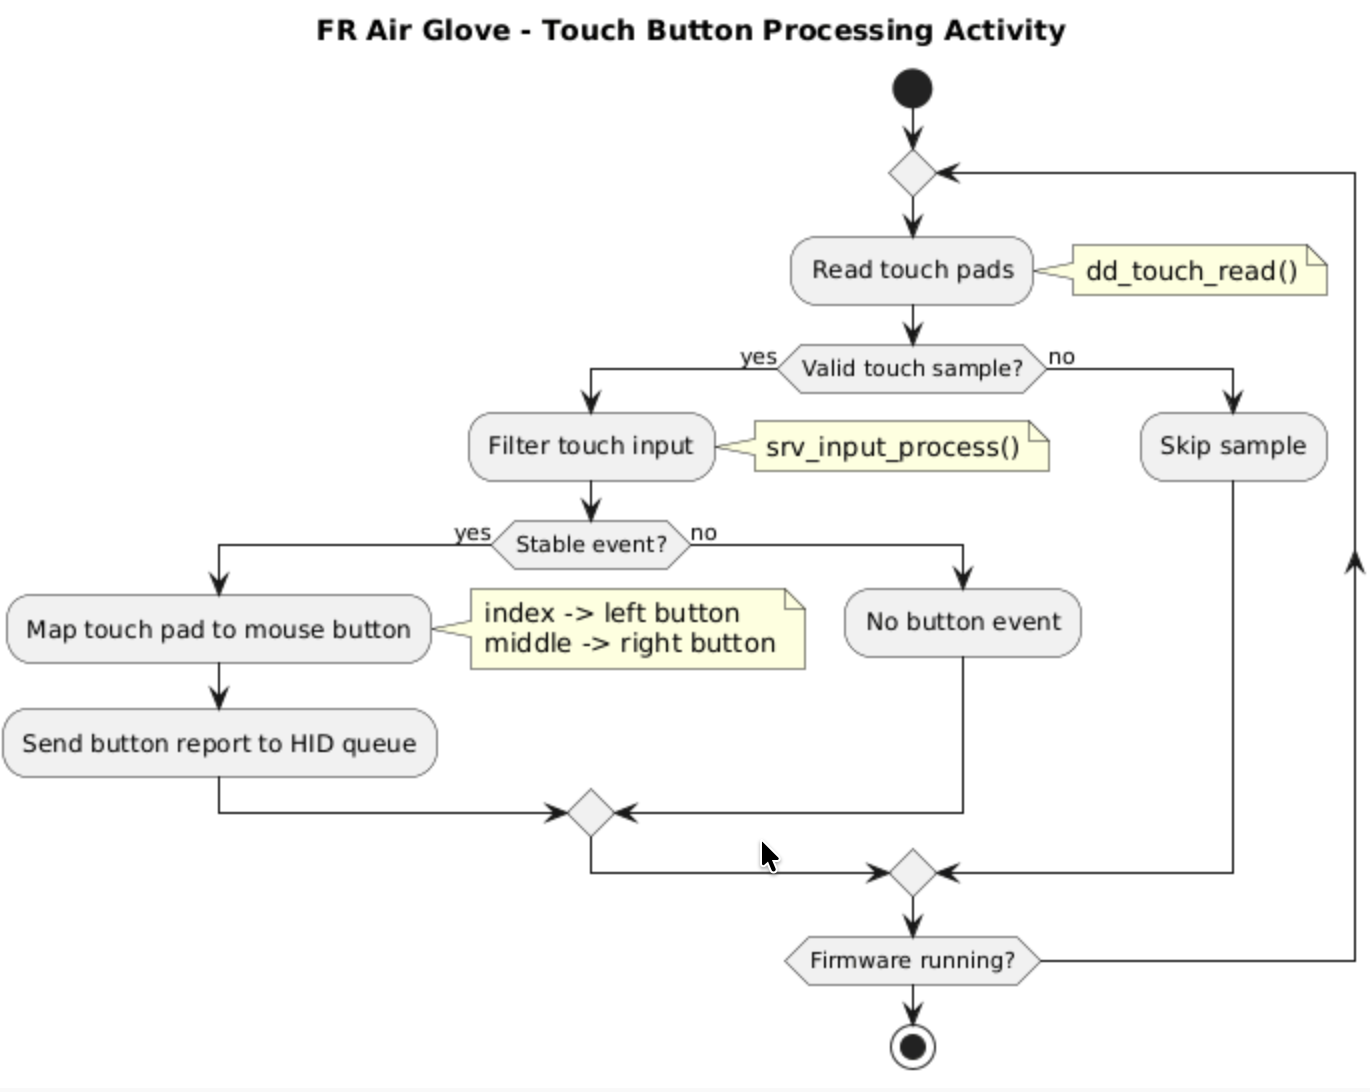
\includegraphics[width=0.5\textwidth]{img/a3.png}
    \caption{FR Air Glove Touch Button Processing Activity Diagram}
    \label{fig:fr-air-glove-activity-touch}
\end{figure}

The touch button processing activity diagram describes how capacitive touch input is converted into mouse button actions. The firmware first reads the touch pads. If the sample is valid, it is passed to the input service, which filters the data and checks whether a stable press or release event occurred.

This filtering step is necessary because capacitive touch values can be noisy. The system should not generate clicks from short glitches or unstable readings. Only stable touch events are mapped to mouse buttons. According to the implemented logic, the index pad is mapped to the left mouse button and the middle pad is mapped to the right mouse button. After mapping, a button report is sent to the HID queue.

If no stable event exists, no button event is produced. If the touch sample is invalid, the firmware skips it and continues running. This activity diagram is useful because it shows how the firmware protects the system from accidental or noisy clicks.

Code support examples:
\begin{itemize}
    \item Touch pads are read using \texttt{dd\_touch\_read()}.
    \item Touch filtering and debounce logic are handled by \texttt{srv\_input\_process()}.
    \item The index touch pad is mapped to the left mouse button.
    \item The middle touch pad is mapped to the right mouse button.
\end{itemize}

\subsubsection{BLE HID Output Activity}

\begin{figure}[H]
    \centering
    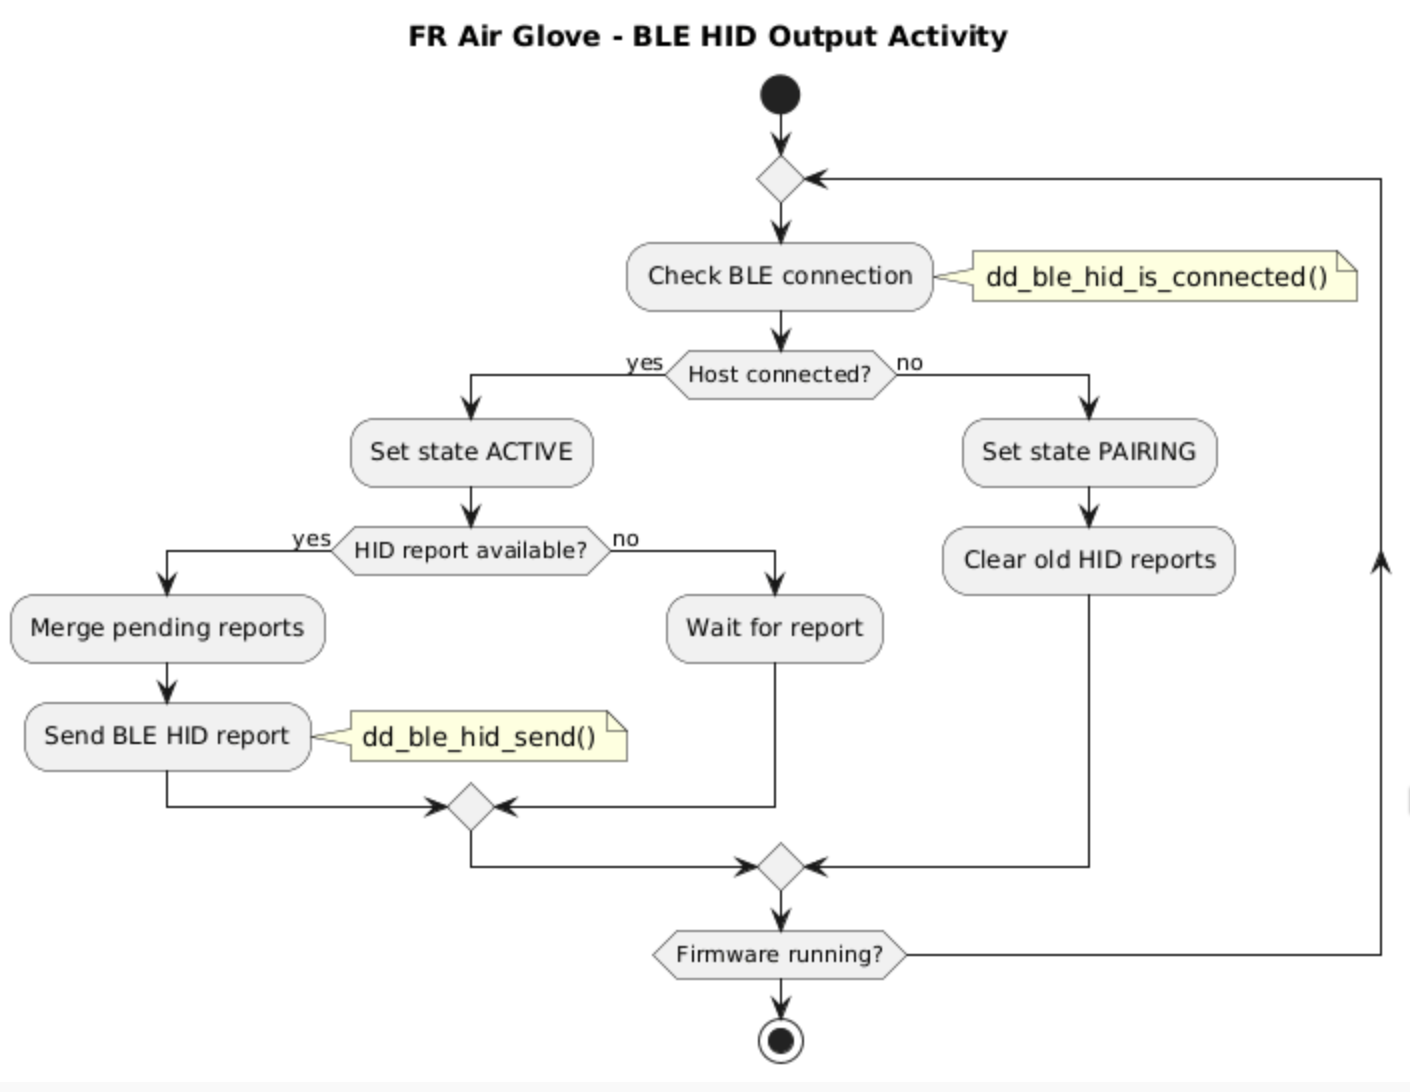
\includegraphics[width=0.5\textwidth]{img/a4.png}
    \caption{FR Air Glove BLE HID Output Activity Diagram}
    \label{fig:fr-air-glove-activity-ble}
\end{figure}

The BLE HID output activity diagram shows how prepared HID reports are sent to the external host. The firmware first checks whether a BLE HID host is connected. If the host is connected, the firmware enters the active state and checks whether a HID report is available. When a report is available, pending reports may be merged, and the final BLE HID report is sent.

If no HID report is available, the firmware waits for the next report. If the host is not connected, the firmware switches to pairing state and clears old HID reports. Clearing old reports is important because movement or click data generated before connection should not be sent later as stale input.

This diagram is useful because it shows that BLE output is controlled by connection state. The glove does not blindly send reports; it first verifies that a host is connected and then sends only valid prepared HID data.

Code support examples:
\begin{itemize}
    \item BLE connection state is checked with \texttt{dd\_ble\_hid\_is\_connected()}.
    \item The active and pairing states correspond to the firmware state logic.
    \item HID reports are represented by \texttt{hid\_mouse\_report\_t}.
    \item BLE transmission is performed using \texttt{dd\_ble\_hid\_send()}.
\end{itemize}

\subsection{Sequence Diagrams}

The sequence diagrams describe interactions between modules over time. They were divided into four smaller diagrams: firmware startup, motion-to-cursor processing, touch-to-button processing, and BLE HID transmission.

\subsubsection{Firmware Startup Sequence}

\begin{figure}[H]
    \centering
    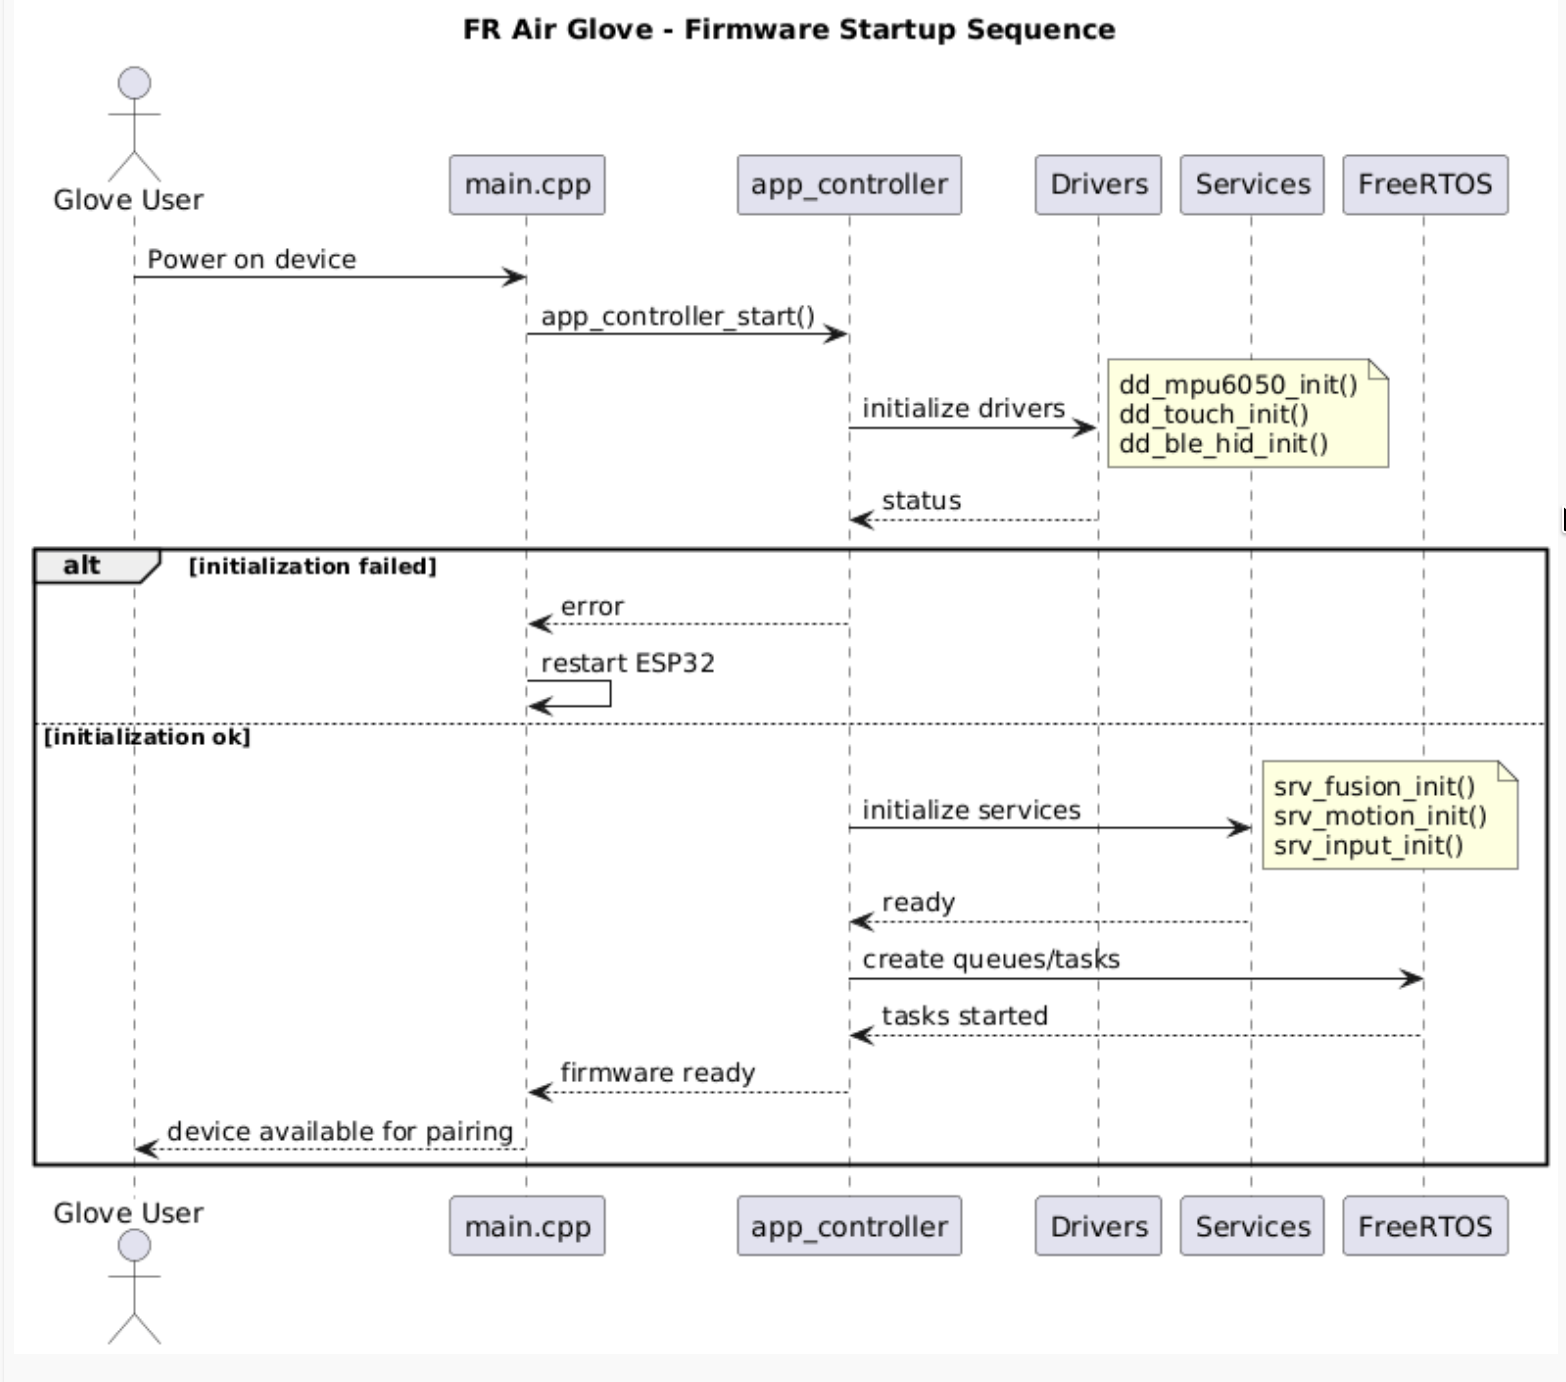
\includegraphics[width=0.5\textwidth]{img/s1.png}
    \caption{FR Air Glove Firmware Startup Sequence Diagram}
    \label{fig:fr-air-glove-sequence-startup}
\end{figure}

The firmware startup sequence diagram shows how the system components interact when the device is powered on. The glove user powers on the ESP32, which starts execution in \texttt{main.cpp}. The main file calls the application controller, and the controller initializes the internal system.

The controller first initializes the hardware drivers. These include the IMU driver, touch driver, and BLE HID driver. The drivers return their status to the controller. If initialization fails, the controller returns an error and the system restarts. If initialization succeeds, the controller continues by initializing services and creating FreeRTOS queues and tasks.

The final result of a successful startup is that the firmware becomes ready and the device becomes available for BLE pairing. This is a realistic representation because the user does not directly receive software messages; instead, the user observes that the device is available through its BLE behavior.

Code support examples:
\begin{itemize}
    \item \texttt{main.cpp} calls \texttt{app\_controller\_start()}.
    \item Driver initialization includes \texttt{dd\_mpu6050\_init()}, \texttt{dd\_touch\_init()}, and \texttt{dd\_ble\_hid\_init()}.
    \item Service initialization includes \texttt{srv\_fusion\_init()}, \texttt{srv\_motion\_init()}, and \texttt{srv\_input\_init()}.
    \item FreeRTOS queues and tasks are created during controller startup.
\end{itemize}

\subsubsection{Motion to Cursor Sequence}

\begin{figure}[H]
    \centering
    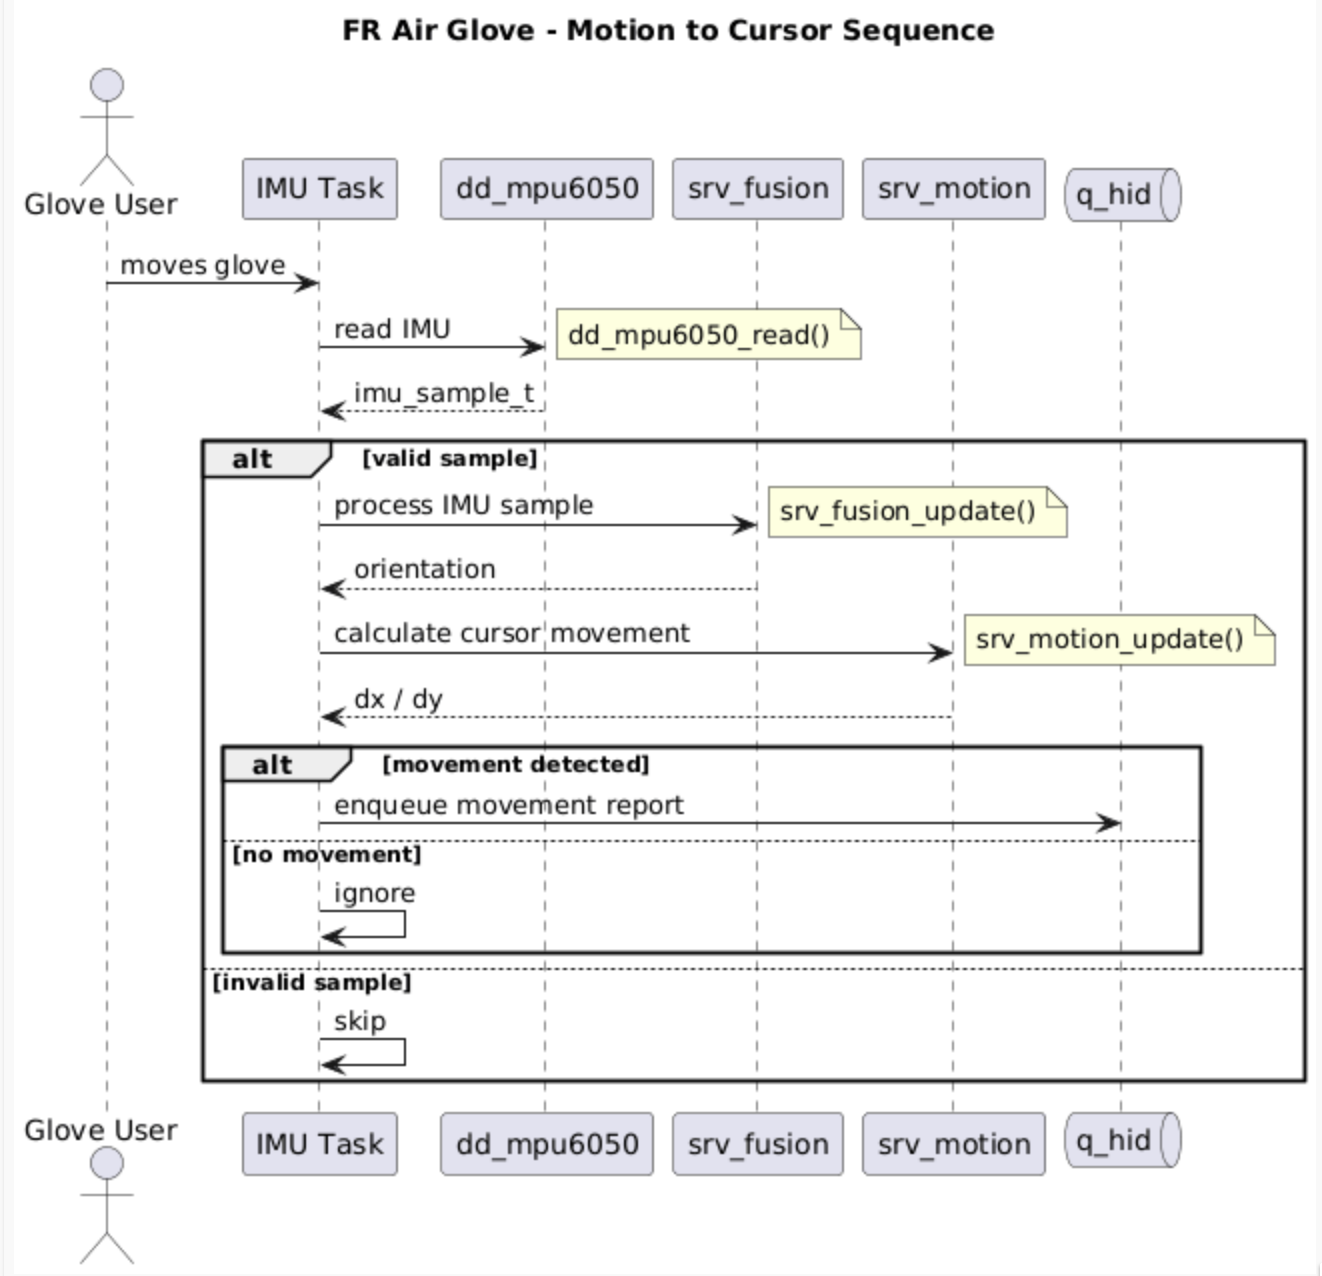
\includegraphics[width=0.5\textwidth]{img/s2.png}
    \caption{FR Air Glove Motion to Cursor Sequence Diagram}
    \label{fig:fr-air-glove-sequence-motion}
\end{figure}

The motion to cursor sequence diagram shows how the user's physical hand movement is transformed into mouse cursor movement. The glove user moves the device, and the IMU task reads motion data using the MPU6050 driver. The driver returns an IMU sample to the task.

If the sample is valid, the data is processed by the fusion service, which estimates the orientation of the glove. This orientation is then passed to the motion service, which calculates cursor movement values such as \texttt{dx} and \texttt{dy}. If movement is detected, a movement report is placed into the HID queue. If no movement is detected, the sample is ignored.

This sequence diagram is useful because it shows that cursor movement is not generated directly from raw sensor values. Instead, the firmware uses a processing chain: sensor reading, orientation estimation, movement calculation, and HID report creation.

Code support examples:
\begin{itemize}
    \item The IMU task reads sensor data using \texttt{dd\_mpu6050\_read()}.
    \item Orientation is estimated using \texttt{srv\_fusion\_update()}.
    \item Cursor movement is calculated using \texttt{srv\_motion\_update()}.
    \item Movement output is sent to the HID queue as a mouse movement report.
\end{itemize}

\subsubsection{Touch to Button Sequence}

\begin{figure}[H]
    \centering
    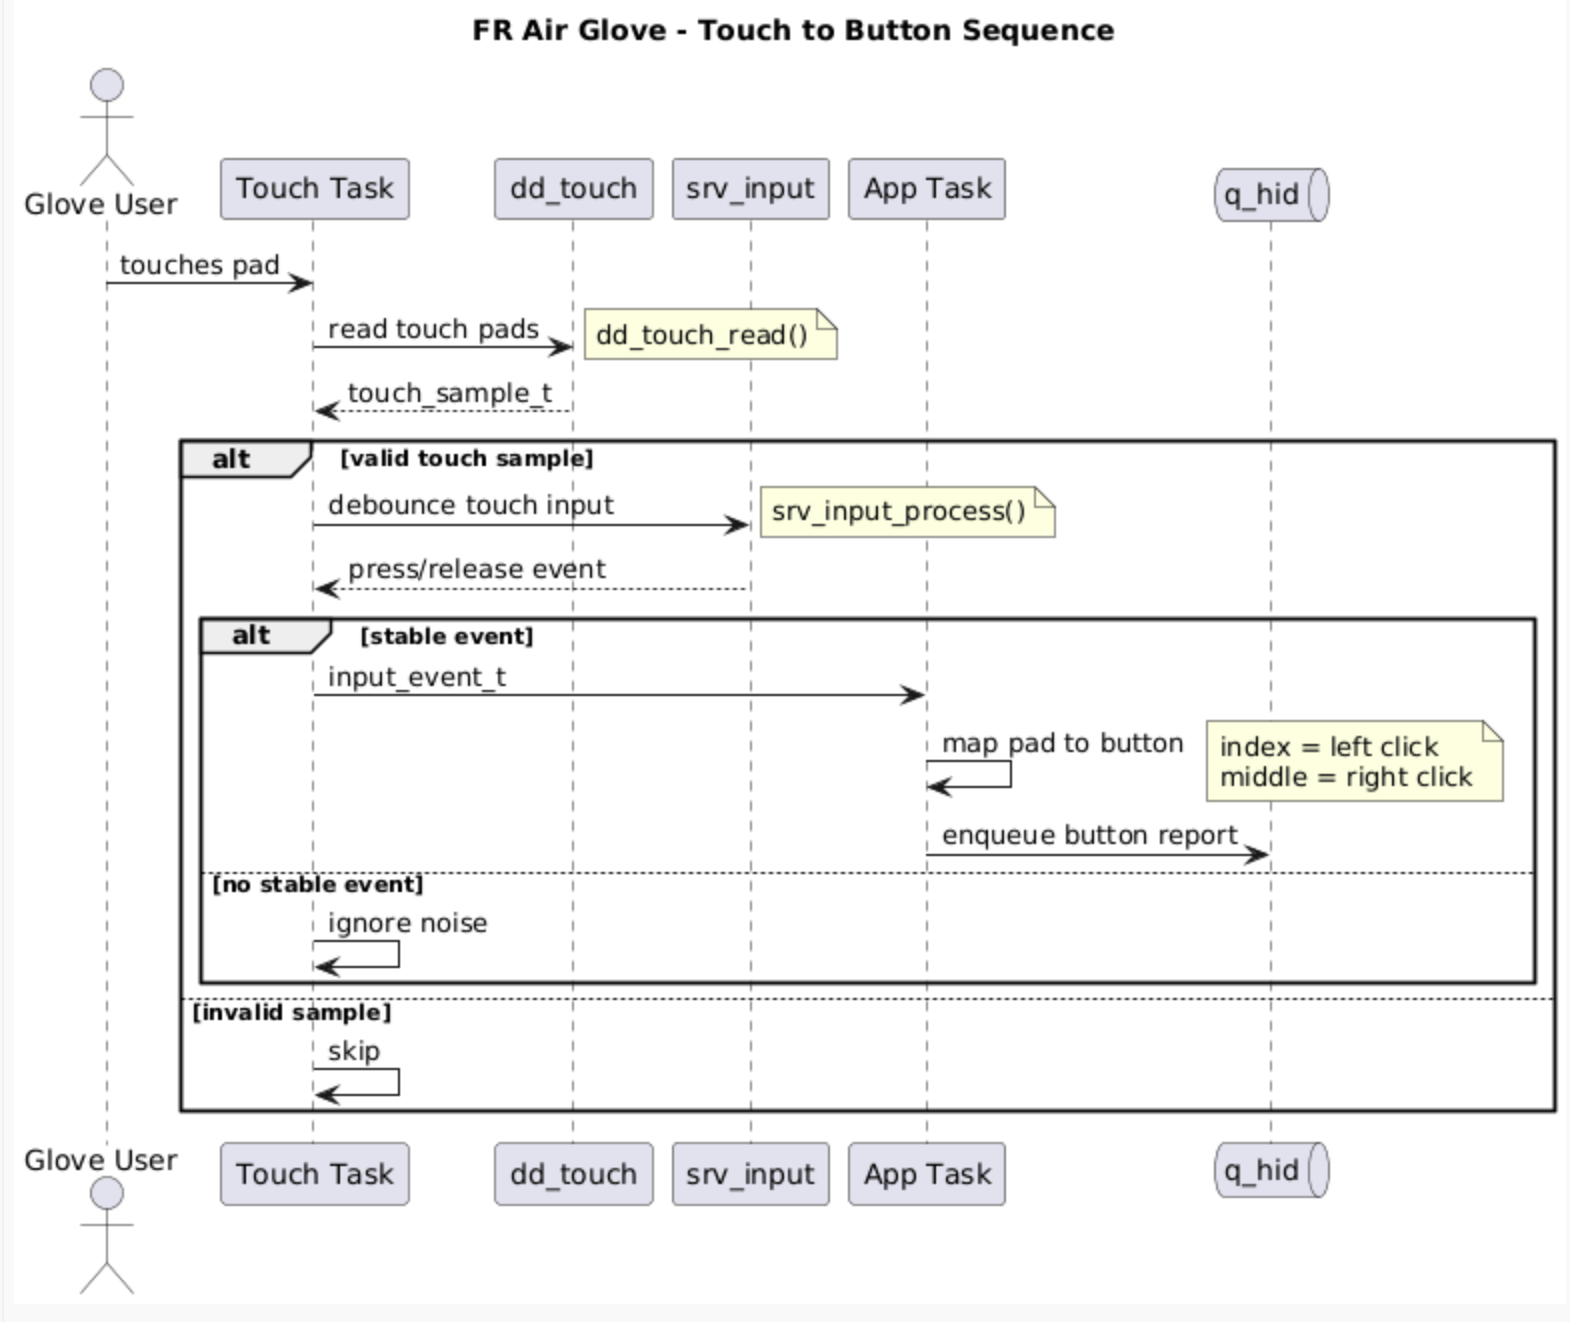
\includegraphics[width=0.5\textwidth]{img/s3.png}
    \caption{FR Air Glove Touch to Button Sequence Diagram}
    \label{fig:fr-air-glove-sequence-touch}
\end{figure}

The touch to button sequence diagram explains how a touch action becomes a mouse button report. The glove user touches one of the capacitive pads, and the touch task reads the pad values through the touch driver. The driver returns a touch sample to the task.

If the sample is valid, the input service processes it and checks whether a stable press or release event exists. This prevents unstable readings from becoming false button clicks. When a stable event is detected, the application task maps the pad to a mouse button. The index pad is mapped to the left click, while the middle pad is mapped to the right click. After mapping, the application task sends a button report to the HID queue.

This sequence diagram is useful because it clearly separates raw touch acquisition from input validation and button mapping. It also shows why the input service is needed before producing HID output.

Code support examples:
\begin{itemize}
    \item Capacitive touch values are read by \texttt{dd\_touch\_read()}.
    \item Touch validation and debounce are handled by \texttt{srv\_input\_process()}.
    \item Stable events are represented as press or release events.
    \item Button reports are sent to the HID queue after pad-to-button mapping.
\end{itemize}

\subsubsection{BLE HID Transmission Sequence}

\begin{figure}[H]
    \centering
    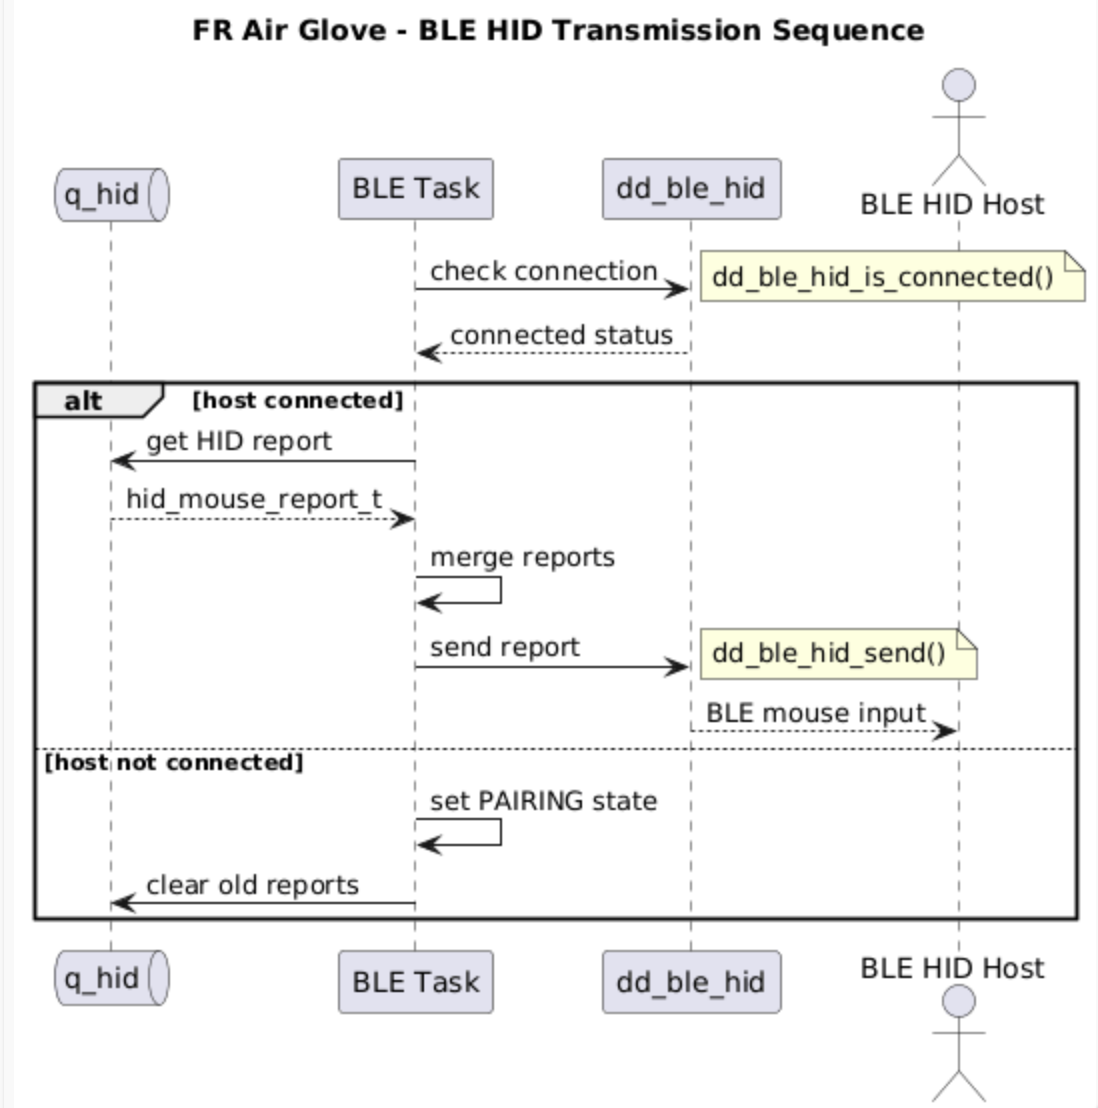
\includegraphics[width=0.5\textwidth]{img/s4.png}
    \caption{FR Air Glove BLE HID Transmission Sequence Diagram}
    \label{fig:fr-air-glove-sequence-ble}
\end{figure}

The BLE HID transmission sequence diagram describes how prepared HID reports are delivered to the external host device. The BLE task first checks the connection state through the BLE HID driver. The driver returns whether a host is connected or not.

If a host is connected, the BLE task reads a HID report from the HID queue. Before sending, it may merge pending reports to reduce unnecessary transmissions and preserve the latest button state. The final report is then sent through the BLE HID driver, and the BLE HID host receives it as mouse input.

If no host is connected, the firmware switches to pairing state and clears old HID reports. This prevents old movement or click data from being sent after a later reconnection.

This sequence diagram is useful because it shows that BLE transmission is isolated in a specific task and driver. Other modules only prepare reports; the BLE task decides when those reports can actually be sent.

Code support examples:
\begin{itemize}
    \item BLE connection is checked using \texttt{dd\_ble\_hid\_is\_connected()}.
    \item HID reports are taken from \texttt{q\_hid}.
    \item Report merging is handled inside the BLE task before sending.
    \item The final report is sent using \texttt{dd\_ble\_hid\_send()}.
\end{itemize}




\addcontentsline{toc}{chapter}{BIBLIOGRAPHY}
\printbibliography[title=BIBLIOGRAPHY]

\appendix

\appendixchapter{Stakeholder Validation Table}
\label{appendix:stakeholder_table}

\begin{table}[!htb]
\caption{Stakeholder Groups and Validation Rationale}
\label{tbl:stakeholders_appendix}
\centering
\begin{tabularx}{\textwidth}{|Y|Y|Y|}
\hline
\textbf{Stakeholder Group} & \textbf{Primary Interest} & \textbf{Validation Signal} \\
\hline
Direct end users (high-exposure computer users) & Reduced cumulative strain and sustainable daily interaction & High MSD and CTS burden with clear exposure-risk links in mouse-intensive work~\cite{demissie2024wrmsd,dale2013cts} \\
\hline
Direct end users (motor-variability populations) & Reliable pointer control under reduced fine-motor stability & Large multi-condition burden and persistent computer-use barriers in arthritis and related groups~\cite{who2022disability,gbd2023oa,baker2009arthritis} \\
\hline
Accessibility and rehabilitation practitioners & Assistive-option evaluation and user-specific adaptation pathways & Documented breakdowns in target acquisition and click stabilisation for motor-impaired users~\cite{wobbrock2008goal} \\
\hline
Educational institutions and presentation-intensive organizations & Surface-independent control for teaching, training, and demonstration scenarios & Recurrent mismatch between fixed-surface assumptions and mobile contexts identified in Chapter~1 \\
\hline
Employers and occupational-health stakeholders & Risk mitigation and productivity preservation in computer-intensive roles & Documented clinical burden with substantial direct and indirect occupational cost exposure~\cite{demissie2024wrmsd,nrc2001msd} \\
\hline
Research and open-source development community & Reproducible platform for algorithmic improvement and accessibility experimentation & Quantified mouse--gyrosensor throughput gap defines a clear optimisation agenda~\cite{ramcharitar2017fitts} \\
\hline
\end{tabularx}
\end{table}
\appendixchapter{Problem Indicators}
\label{appendix:problem_indicators}

\begin{table}[H]
  \caption{Quantitative Evidence Supporting the Need for Alternative Input Approaches}
  \label{tbl:problem_indicators}
  \begin{tabularx}{\textwidth}{|Y|Y|Y|}
    \hline
    \textbf{Dimension} & \textbf{Evidence} & \textbf{Interpretation} \\
    \hline
    Population burden & Work-related MSD prevalence among computer users: 33.8\%--95.3\%~\cite{demissie2024wrmsd} & The risk profile is broad and persistent across user groups. \\
    \hline
    Global trajectory & MSD cases increased 123.4\% (1990--2020), with continued growth projected~\cite{gbd2023othermsd} & The problem scale is increasing, not stabilising. \\
    \hline
    Biomechanical exposure & Mouse use $>$50\% of work time increases hand/wrist symptom odds ratio (OR) to 1.68~\cite{andersen2003mouse} & High-exposure workflows amplify cumulative upper-limb risk. \\
    \hline
    Clinical signal & CTS prevalence 7.8\% in pooled occupational data~\cite{dale2013cts} & A major musculoskeletal outcome is measurable in occupational populations. \\
    \hline
    Accessibility barrier & 85\% of arthritis participants report major computer-use difficulties~\cite{baker2009arthritis} & Classical input assumptions do not generalise across motor conditions. \\
    \hline
    Interaction performance gap & Fitts' law throughput: mouse 4.73~bits/second (bps) vs.\ gyrosensor 2.85~bps~\cite{ramcharitar2017fitts} & Spatial alternatives are viable but require algorithmic refinement to approach parity. \\
    \hline
  \end{tabularx}
\end{table}
\appendixchapter{Comparative Analysis}
\label{appendix:comparative_table}

\begin{table}[H]
\caption{SWOT Analysis of the Proposed Air Mouse Glove}
\label{tbl:swot}
\begin{tabularx}{\textwidth}{|Y|Y|}
\hline
\textbf{Strengths} & \textbf{Weaknesses} \\
\hline
\begin{itemize}[leftmargin=*, labelsep=0.4em]
    \item The glove-style design of the product can feel more comfortable and natural for pointing or clicking compared to a traditional remote, especially for presenters and lecturers;
    \item The hardware components, particularly the ESP32 and MPU6050/6500 sensors, are widely available and reasonably priced compared to commercial wearables;
    \item Similar to an air mouse, the glove benefits from the fact that no desk surface is needed. Midair cursor control is a popular use case for presentations and media control \cite{youtube_airmouse_demo,cornell_airmouse_project};
    \item Many commercial air mice rely on 2.4~GHz communication with a USB receiver \cite{airmouse_y10l,amazon_imouse_p30}, whereas the proposed solution is designed to operate primarily as a Bluetooth HID device, improving portability. A 2.4 GHz alternative remains a potential extension when Bluetooth compatibility or latency becomes a constraint.
\end{itemize}
&
\begin{itemize}[leftmargin=*, labelsep=0.4em]
    \item The MPU6050 sensor (gyroscope and accelerometer) is prone to drift, increasing calibration complexity \cite{gesture_hci_research}. Stable cursor control requires filtering, calibration routines, and careful mapping to screen movement;
    \item Users may require an adaptation period to learn how the device functions (special movements for scrolling, zooming, etc.);
    \item Ergonomics and comfort, such as glove fit, heat, weight distribution, and sensor placement, strongly influence user experience. An uncomfortable device is unlikely to be adopted;
    \item Wearable devices must be reliable in terms of battery life, which remains a common concern among commercial air mouse products.
\end{itemize}
\\
\hline
\textbf{Opportunities} & \textbf{Threats} \\
\hline
\begin{itemize}[leftmargin=*, labelsep=0.4em]
    \item A clear market gap exists, as users frequently complain about the air mouse experience, describing commercial remotes as cheap or inconsistent \cite{reddit_airmouse_discussion};
    \item Existing demand for air mice (presenter remotes, laser pointers) indicates market interest and validates the use case;
    \item Wearable midair control solutions can support users who struggle with traditional mice or trackpads, improving accessibility and ergonomic interaction \cite{acm_airmouse_interface,arxiv_gesture_recognition};
    \item Existing features such as gestures (zoom, scroll), pause mode, and programmable buttons can be further enhanced in the proposed design \cite{gesture_market}.
\end{itemize}
&
\begin{itemize}[leftmargin=*, labelsep=0.4em]
    \item Cheaper commercial alternatives already exist (e.g., approximately 170~Lei for G10S and 349~MDL for C120 in Moldova \cite{antena_airmouse,mshop_airmouse_c120}), making price competition challenging;
    \item Many commercial devices use newer IMUs and optimized firmware, which may provide smoother calibration than an early-stage prototype;
    \item Users have high expectations for precision; shaky, overly sensitive, or laggy cursor behavior can lead to poor user adoption;
    \item Ecosystem compatibility represents a risk, as differences in operating systems and Bluetooth stack implementations may result in inconsistent behavior.
\end{itemize}
\\
\hline
\end{tabularx}
\end{table}









\small
\renewcommand{\arraystretch}{1.25}
\rowcolors{2}{gray!8}{white}

\begin{longtable}{|p{2.9cm}|p{2.35cm}|p{2.35cm}|p{2.35cm}|p{2.35cm}|p{2.35cm}|}
\caption{Comparative Analysis of Existing Solutions and the Proposed Air Mouse Glove}
\label{tbl:comparative_air_mouse} \\
\hline
\rowcolor{gray!20}
\textbf{Criterion} &
\textbf{Presenter Air Mouse (Y-10L)\cite{airmouse_y10l}} &
\textbf{Commercial Air Mouse (G10S / C120)\cite{antena_airmouse,mshop_airmouse_c120}} &
\textbf{Wearable Concepts (Ion, Bellcos)\cite{ergonomic_airmouse_glove,bellcos_wireless_mouse}} &
\textbf{Research / DIY Glove Projects\cite{cornell_airmouse_project,youtube_airmouse_demo}} &
\textbf{Proposed Air Mouse Glove (ESP32 + MPU6050/6500)} \\
\hline
\endfirsthead

\hline
\rowcolor{gray!20}
\textbf{Criterion} &
\textbf{Presenter Air Mouse (Y-10L)} &
\textbf{Commercial Air Mouse} &
\textbf{Wearable Concepts} &
\textbf{Research / DIY Projects} &
\textbf{Proposed Air Mouse Glove} \\
\hline
\endhead

\textbf{Form Factor / Wearability} &
Handheld presenter with buttons and trackball &
Handheld remote &
Wearable glove or partial glove &
Full glove or prototype wearable &
Wearable glove \\
\hline

\textbf{Interaction Method} &
Trackball + buttons &
Tilt-based motion + buttons &
Hand motion and gestures &
Hand motion, gestures &
Hand motion, gestures, buttons \\
\hline

\textbf{Sensor Technology} &
Optical + inertial sensors &
IMU (gyro + accelerometer) &
IMU-based motion tracking &
IMU (gyro + accel) &
MPU6050 / MPU6500 IMU \\
\hline

\textbf{Connectivity Method} &
2.4~GHz USB receiver &
2.4~GHz USB receiver &
Wireless (varies) &
Wired or wireless (custom) &
Bluetooth HID (ESP32) — primary (2.4 GHz optional variant) \\
\hline

\textbf{Precision \& Stability} &
Medium--high (trackball assisted) &
Medium (often jittery) &
Variable, experimental &
Variable, algorithm-dependent &
Tunable via filtering \& sensor fusion \\
\hline

\textbf{Calibration \& Algorithms} &
Factory-calibrated &
Minimal or automatic &
Limited or experimental &
Custom filtering \& calibration &
Complementary/ Kalman filters, calibration routines \\
\hline

\textbf{Ease of Use / Learning Curve} &
Easy, intuitive &
Moderate &
Moderate to high &
High (technical setup) &
Moderate \\
\hline

\textbf{Portability} &
Requires USB dongle &
Requires USB dongle &
Wireless, device-dependent &
Limited &
High (no dongle required) \\
\hline

\textbf{Target Use Case} &
Presentations, lectures &
Media control, HTPC &
Experimental / niche use &
Academic research &
Presentations, accessibility, research \\
\hline

\textbf{Cost / Availability} &
Commercial, mid-range price &
Commercial, low cost &
Rare / discontinued &
Not commercial &
Low-cost prototype \\
\hline

\textbf{Battery Life / Power} &
USB-powered / internal battery (varies by model) &
Often limited ($\sim$8--12~h reported); common user complaint &
Not specified / device-dependent &
External power &
Dependent on ESP32 LiPo configuration; optimisable via deep-sleep modes \\
\hline

\textbf{Open-Source / Customisability} &
Closed, proprietary firmware &
Closed, proprietary firmware &
Limited / undocumented &
Fully open; firmware adjustable &
Fully open; ESP32 Arduino/IDF ecosystem with open-source libraries \\
\hline

\end{longtable}

% \appendixchapter{Some code}
% \label{appendix:bucket_call}

% \begin{listing}[ht]
% \inputminted{js}{src/code.js}
% \end{listing}


\end{document}